\documentclass[1p]{elsarticle_modified}
%\bibliographystyle{elsarticle-num}

%\usepackage[colorlinks]{hyperref}
%\usepackage{abbrmath_seonhwa} %\Abb, \Ascr, \Acal ,\Abf, \Afrak
\usepackage{amsfonts}
\usepackage{amssymb}
\usepackage{amsmath}
\usepackage{amsthm}
\usepackage{scalefnt}
\usepackage{amsbsy}
\usepackage{kotex}
\usepackage{caption}
\usepackage{subfig}
\usepackage{color}
\usepackage{graphicx}
\usepackage{xcolor} %% white, black, red, green, blue, cyan, magenta, yellow
\usepackage{float}
\usepackage{setspace}
\usepackage{hyperref}

\usepackage{tikz}
\usetikzlibrary{arrows}

\usepackage{multirow}
\usepackage{array} % fixed length table
\usepackage{hhline}

%%%%%%%%%%%%%%%%%%%%%
\makeatletter
\renewcommand*\env@matrix[1][\arraystretch]{%
	\edef\arraystretch{#1}%
	\hskip -\arraycolsep
	\let\@ifnextchar\new@ifnextchar
	\array{*\c@MaxMatrixCols c}}
\makeatother %https://tex.stackexchange.com/questions/14071/how-can-i-increase-the-line-spacing-in-a-matrix
%%%%%%%%%%%%%%%

\usepackage[normalem]{ulem}

\newcommand{\msout}[1]{\ifmmode\text{\sout{\ensuremath{#1}}}\else\sout{#1}\fi}
%SOURCE: \msout is \stkout macro in https://tex.stackexchange.com/questions/20609/strikeout-in-math-mode

\newcommand{\cancel}[1]{
	\ifmmode
	{\color{red}\msout{#1}}
	\else
	{\color{red}\sout{#1}}
	\fi
}

\newcommand{\add}[1]{
	{\color{blue}\uwave{#1}}
}

\newcommand{\replace}[2]{
	\ifmmode
	{\color{red}\msout{#1}}{\color{blue}\uwave{#2}}
	\else
	{\color{red}\sout{#1}}{\color{blue}\uwave{#2}}
	\fi
}

\newcommand{\Sol}{\mathcal{S}} %segment
\newcommand{\D}{D} %diagram
\newcommand{\A}{\mathcal{A}} %arc


%%%%%%%%%%%%%%%%%%%%%%%%%%%%%5 test

\def\sl{\operatorname{\textup{SL}}(2,\Cbb)}
\def\psl{\operatorname{\textup{PSL}}(2,\Cbb)}
\def\quan{\mkern 1mu \triangleright \mkern 1mu}

\theoremstyle{definition}
\newtheorem{thm}{Theorem}[section]
\newtheorem{prop}[thm]{Proposition}
\newtheorem{lem}[thm]{Lemma}
\newtheorem{ques}[thm]{Question}
\newtheorem{cor}[thm]{Corollary}
\newtheorem{defn}[thm]{Definition}
\newtheorem{exam}[thm]{Example}
\newtheorem{rmk}[thm]{Remark}
\newtheorem{alg}[thm]{Algorithm}

\newcommand{\I}{\sqrt{-1}}
\begin{document}

%\begin{frontmatter}
%
%\title{Boundary parabolic representations of knots up to 8 crossings}
%
%%% Group authors per affiliation:
%\author{Yunhi Cho} 
%\address{Department of Mathematics, University of Seoul, Seoul, Korea}
%\ead{yhcho@uos.ac.kr}
%
%
%\author{Seonhwa Kim} %\fnref{s_kim}}
%\address{Center for Geometry and Physics, Institute for Basic Science, Pohang, 37673, Korea}
%\ead{ryeona17@ibs.re.kr}
%
%\author{Hyuk Kim}
%\address{Department of Mathematical Sciences, Seoul National University, Seoul 08826, Korea}
%\ead{hyukkim@snu.ac.kr}
%
%\author{Seokbeom Yoon}
%\address{Department of Mathematical Sciences, Seoul National University, Seoul, 08826,  Korea}
%\ead{sbyoon15@snu.ac.kr}
%
%\begin{abstract}
%We find all boundary parabolic representation of knots up to 8 crossings.
%
%\end{abstract}
%\begin{keyword}
%    \MSC[2010] 57M25 
%\end{keyword}
%
%\end{frontmatter}

%\linenumbers
%\tableofcontents
%
\newcommand\colored[1]{\textcolor{white}{\rule[-0.35ex]{0.8em}{1.4ex}}\kern-0.8em\color{red} #1}%
%\newcommand\colored[1]{\textcolor{white}{ #1}\kern-2.17ex	\textcolor{white}{ #1}\kern-1.81ex	\textcolor{white}{ #1}\kern-2.15ex\color{red}#1	}

{\Large $\underline{12a_{0897}~(K12a_{0897})}$}

\setlength{\tabcolsep}{10pt}
\renewcommand{\arraystretch}{1.6}
\vspace{1cm}\begin{tabular}{m{100pt}>{\centering\arraybackslash}m{274pt}}
\multirow{5}{120pt}{
	\centering
	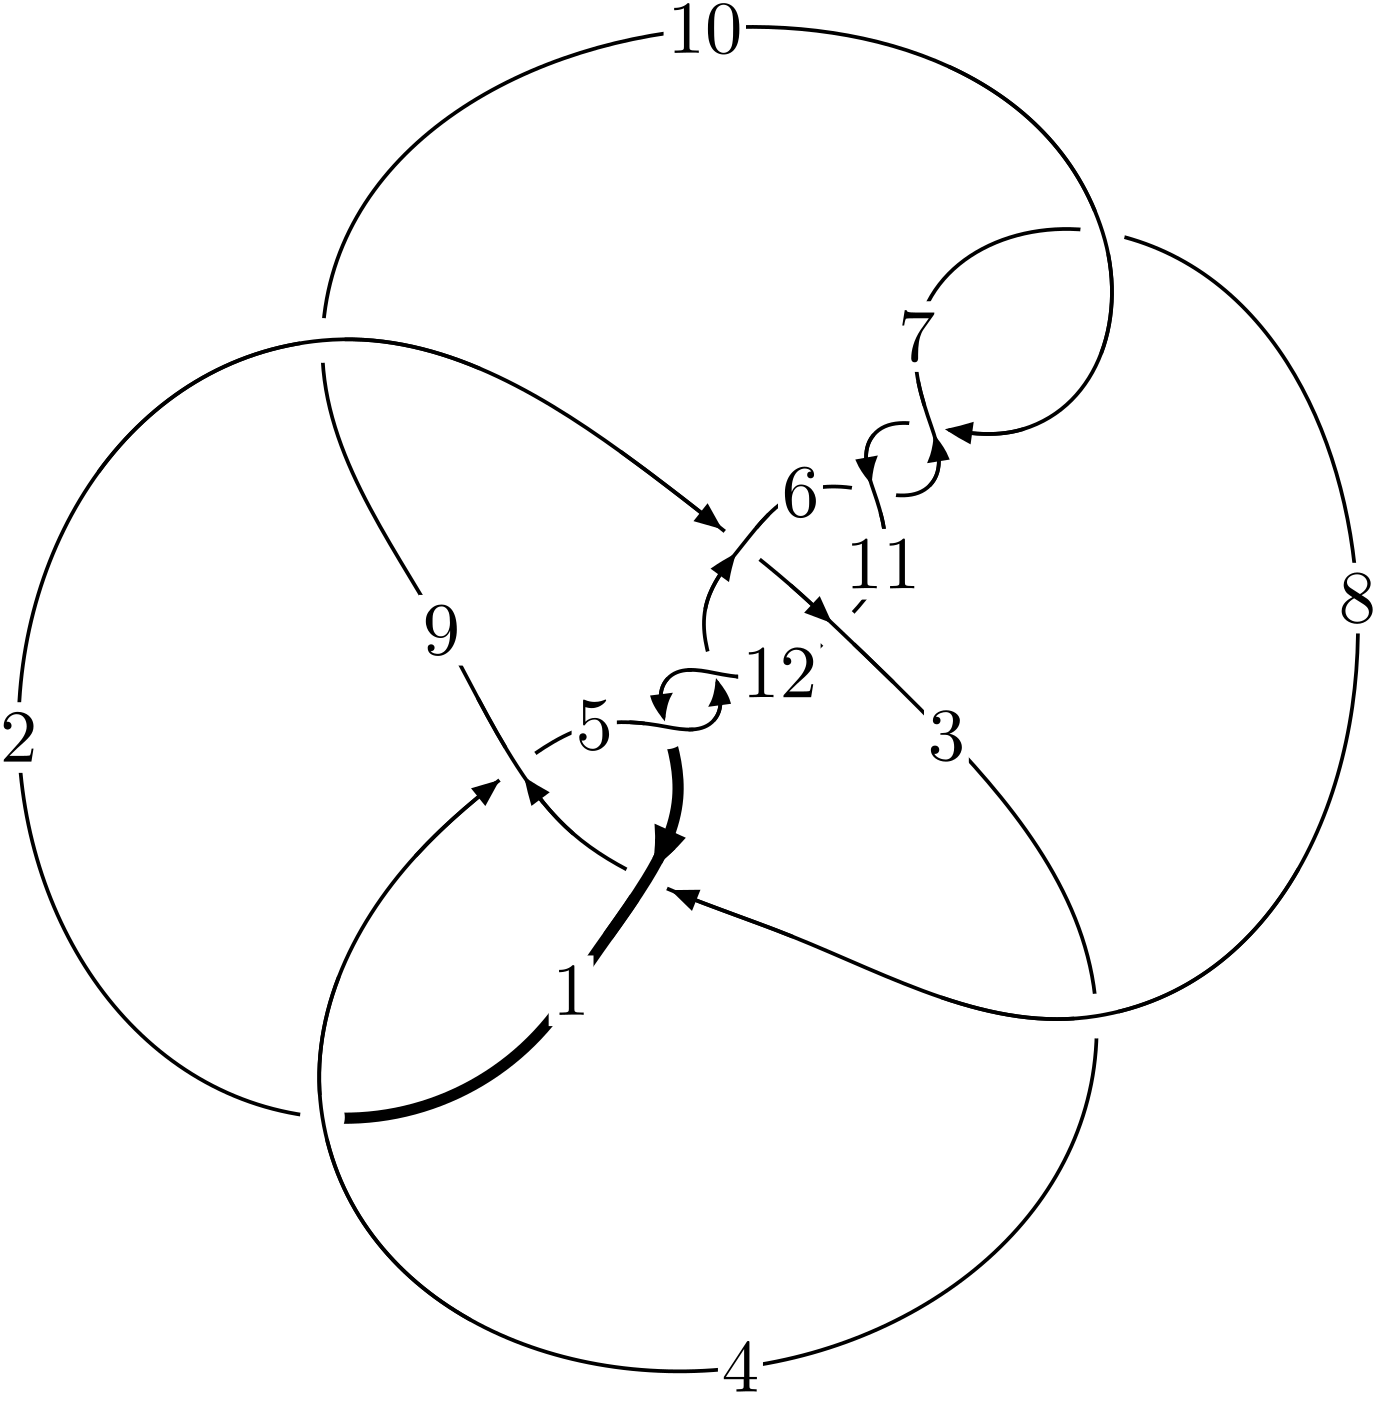
\includegraphics[width=112pt]{../../../GIT/diagram.site/Diagrams/png/1698_12a_0897.png}\\
\ \ \ A knot diagram\footnotemark}&
\allowdisplaybreaks
\textbf{Linearized knot diagam} \\
\cline{2-2}
 &
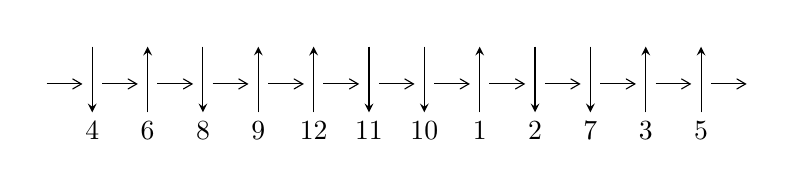
\begin{tikzpicture}[x=20pt, y=17pt]
	% nodes
	\node (C0) at (0, 0) {};
	\node (C1) at (1, 0) {};
	\node (C1U) at (1, +1) {};
	\node (C1D) at (1, -1) {4};

	\node (C2) at (2, 0) {};
	\node (C2U) at (2, +1) {};
	\node (C2D) at (2, -1) {6};

	\node (C3) at (3, 0) {};
	\node (C3U) at (3, +1) {};
	\node (C3D) at (3, -1) {8};

	\node (C4) at (4, 0) {};
	\node (C4U) at (4, +1) {};
	\node (C4D) at (4, -1) {9};

	\node (C5) at (5, 0) {};
	\node (C5U) at (5, +1) {};
	\node (C5D) at (5, -1) {12};

	\node (C6) at (6, 0) {};
	\node (C6U) at (6, +1) {};
	\node (C6D) at (6, -1) {11};

	\node (C7) at (7, 0) {};
	\node (C7U) at (7, +1) {};
	\node (C7D) at (7, -1) {10};

	\node (C8) at (8, 0) {};
	\node (C8U) at (8, +1) {};
	\node (C8D) at (8, -1) {1};

	\node (C9) at (9, 0) {};
	\node (C9U) at (9, +1) {};
	\node (C9D) at (9, -1) {2};

	\node (C10) at (10, 0) {};
	\node (C10U) at (10, +1) {};
	\node (C10D) at (10, -1) {7};

	\node (C11) at (11, 0) {};
	\node (C11U) at (11, +1) {};
	\node (C11D) at (11, -1) {3};

	\node (C12) at (12, 0) {};
	\node (C12U) at (12, +1) {};
	\node (C12D) at (12, -1) {5};
	\node (C13) at (13, 0) {};

	% arrows
	\draw[->,>={angle 60}]
	(C0) edge (C1) (C1) edge (C2) (C2) edge (C3) (C3) edge (C4) (C4) edge (C5) (C5) edge (C6) (C6) edge (C7) (C7) edge (C8) (C8) edge (C9) (C9) edge (C10) (C10) edge (C11) (C11) edge (C12) (C12) edge (C13) ;	\draw[->,>=stealth]
	(C1U) edge (C1D) (C2D) edge (C2U) (C3U) edge (C3D) (C4D) edge (C4U) (C5D) edge (C5U) (C6U) edge (C6D) (C7U) edge (C7D) (C8D) edge (C8U) (C9U) edge (C9D) (C10U) edge (C10D) (C11D) edge (C11U) (C12D) edge (C12U) ;
	\end{tikzpicture} \\
\hhline{~~} \\& 
\textbf{Solving Sequence} \\ \cline{2-2} 
 &
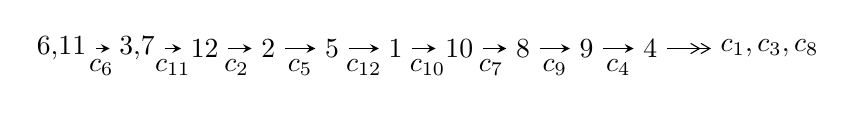
\begin{tikzpicture}[x=23pt, y=7pt]
	% node
	\node (A0) at (-1/8, 0) {6,11};
	\node (A1) at (17/16, 0) {3,7};
	\node (A2) at (17/8, 0) {12};
	\node (A3) at (25/8, 0) {2};
	\node (A4) at (33/8, 0) {5};
	\node (A5) at (41/8, 0) {1};
	\node (A6) at (49/8, 0) {10};
	\node (A7) at (57/8, 0) {8};
	\node (A8) at (65/8, 0) {9};
	\node (A9) at (73/8, 0) {4};
	\node (C1) at (1/2, -1) {$c_{6}$};
	\node (C2) at (13/8, -1) {$c_{11}$};
	\node (C3) at (21/8, -1) {$c_{2}$};
	\node (C4) at (29/8, -1) {$c_{5}$};
	\node (C5) at (37/8, -1) {$c_{12}$};
	\node (C6) at (45/8, -1) {$c_{10}$};
	\node (C7) at (53/8, -1) {$c_{7}$};
	\node (C8) at (61/8, -1) {$c_{9}$};
	\node (C9) at (69/8, -1) {$c_{4}$};
	\node (A10) at (11, 0) {$c_{1},c_{3},c_{8}$};

	% edge
	\draw[->,>=stealth]	
	(A0) edge (A1) (A1) edge (A2) (A2) edge (A3) (A3) edge (A4) (A4) edge (A5) (A5) edge (A6) (A6) edge (A7) (A7) edge (A8) (A8) edge (A9) ;
	\draw[->>,>={angle 60}]	
	(A9) edge (A10);
\end{tikzpicture} \\ 

\end{tabular} \\

\footnotetext{
The image of knot diagram is generated by the software ``\textbf{Draw programme}" developed by Andrew Bartholomew(\url{http://www.layer8.co.uk/maths/draw/index.htm\#Running-draw}), where we modified some parts for our purpose(\url{https://github.com/CATsTAILs/LinksPainter}).
}\phantom \\ \newline 
\centering \textbf{Ideals for irreducible components\footnotemark of $X_{\text{par}}$} 
 
\begin{align*}
I^u_{1}&=\langle 
57881957452448 u^{41}+869354193740770 u^{40}+\cdots+35295682071297 b-13155101208038300,\\
\phantom{I^u_{1}}&\phantom{= \langle  }1.31551\times10^{16} u^{41}+1.76547\times10^{17} u^{40}+\cdots+1.26711\times10^{16} a-8.53632\times10^{17},\\
\phantom{I^u_{1}}&\phantom{= \langle  }u^{42}+15 u^{41}+\cdots-7744 u-359\rangle \\
I^u_{2}&=\langle 
-1.04951\times10^{13} a^{5} u^{14}+2.29419\times10^{15} a^{4} u^{14}+\cdots-1.07487\times10^{15} a-3.31910\times10^{15},\\
\phantom{I^u_{2}}&\phantom{= \langle  }- u^{14} a^5+3 u^{14} a^4+\cdots-48 a-192,\\
\phantom{I^u_{2}}&\phantom{= \langle  }u^{15}-3 u^{14}+12 u^{13}-25 u^{12}+52 u^{11}-78 u^{10}+104 u^9-109 u^8+94 u^7-58 u^6+24 u^5+2 u^4-8 u^3+4 u^2-1\rangle \\
I^u_{3}&=\langle 
23 u^{22}+100 u^{21}+\cdots+623 b-207,\;-207 u^{22}+1058 u^{21}+\cdots+623 a+1151,\\
\phantom{I^u_{3}}&\phantom{= \langle  }u^{23}-5 u^{22}+\cdots-2 u-1\rangle \\
I^u_{4}&=\langle 
u^3+b+u,\;u^2+a+1,\;u^4- u^3+2 u^2-2 u+1\rangle \\
\\
I^v_{1}&=\langle 
a,\;b^3+b^2-1,\;v-1\rangle \\
\end{align*}
\raggedright * 5 irreducible components of $\dim_{\mathbb{C}}=0$, with total 162 representations.\\
\footnotetext{All coefficients of polynomials are rational numbers. But the coefficients are sometimes approximated in decimal forms when there is not enough margin.}
\newpage
\renewcommand{\arraystretch}{1}
\centering \section*{I. $I^u_{1}= \langle 5.79\times10^{13} u^{41}+8.69\times10^{14} u^{40}+\cdots+3.53\times10^{13} b-1.32\times10^{16},\;1.32\times10^{16} u^{41}+1.77\times10^{17} u^{40}+\cdots+1.27\times10^{16} a-8.54\times10^{17},\;u^{42}+15 u^{41}+\cdots-7744 u-359 \rangle$}
\flushleft \textbf{(i) Arc colorings}\\
\begin{tabular}{m{7pt} m{180pt} m{7pt} m{180pt} }
\flushright $a_{6}=$&$\begin{pmatrix}1\\0\end{pmatrix}$ \\
\flushright $a_{11}=$&$\begin{pmatrix}0\\u\end{pmatrix}$ \\
\flushright $a_{3}=$&$\begin{pmatrix}-1.03819 u^{41}-13.9330 u^{40}+\cdots+1261.90 u+67.3681\\-1.63992 u^{41}-24.6306 u^{40}+\cdots+7972.40 u+372.711\end{pmatrix}$ \\
\flushright $a_{7}=$&$\begin{pmatrix}1\\u^2\end{pmatrix}$ \\
\flushright $a_{12}=$&$\begin{pmatrix}0.173456 u^{41}+3.15349 u^{40}+\cdots-143.162 u-6.32280\\-0.551641 u^{41}-6.89586 u^{40}+\cdots-1335.92 u-62.2709\end{pmatrix}$ \\
\flushright $a_{2}=$&$\begin{pmatrix}0.601723 u^{41}+10.6976 u^{40}+\cdots-6710.50 u-305.343\\-1.63992 u^{41}-24.6306 u^{40}+\cdots+7972.40 u+372.711\end{pmatrix}$ \\
\flushright $a_{5}=$&$\begin{pmatrix}-1.57357 u^{41}-21.8016 u^{40}+\cdots-1184.91 u-54.6381\\-0.423171 u^{41}-8.96377 u^{40}+\cdots+7907.19 u+366.873\end{pmatrix}$ \\
\flushright $a_{1}=$&$\begin{pmatrix}0.557687 u^{41}+4.38234 u^{40}+\cdots+10797.2 u+500.615\\2.74550 u^{41}+42.6628 u^{40}+\cdots-12062.7 u-550.167\end{pmatrix}$ \\
\flushright $a_{10}=$&$\begin{pmatrix}u\\u^3+u\end{pmatrix}$ \\
\flushright $a_{8}=$&$\begin{pmatrix}u^2+1\\u^4+2 u^2\end{pmatrix}$ \\
\flushright $a_{9}=$&$\begin{pmatrix}0.679616 u^{41}+10.3741 u^{40}+\cdots-3056.20 u-144.610\\-0.584616 u^{41}-8.36449 u^{40}+\cdots-555.966 u-34.1050\end{pmatrix}$ \\
\flushright $a_{4}=$&$\begin{pmatrix}-0.952487 u^{41}-14.7913 u^{40}+\cdots+6842.37 u+332.671\\0.555898 u^{41}+7.29831 u^{40}+\cdots-374.764 u-12.6868\end{pmatrix}$\\&\end{tabular}
\flushleft \textbf{(ii) Obstruction class $= -1$}\\~\\
\flushleft \textbf{(iii) Cusp Shapes $= -\frac{56056292405896}{11765227357099} u^{41}-\frac{807397111618689}{11765227357099} u^{40}+\cdots+\frac{169436635472717727}{11765227357099} u+\frac{8474387662208614}{11765227357099}$}\\~\\
\newpage\renewcommand{\arraystretch}{1}
\flushleft \textbf{(iv) u-Polynomials at the component}\newline \\
\begin{tabular}{m{50pt}|m{274pt}}
Crossings & \hspace{64pt}u-Polynomials at each crossing \\
\hline $$\begin{aligned}c_{1}\end{aligned}$$&$\begin{aligned}
&u^{42}-32 u^{41}+\cdots+4335 u-359
\end{aligned}$\\
\hline $$\begin{aligned}c_{2},c_{11}\end{aligned}$$&$\begin{aligned}
&u^{42}- u^{41}+\cdots+u-1
\end{aligned}$\\
\hline $$\begin{aligned}c_{3},c_{9}\end{aligned}$$&$\begin{aligned}
&u^{42}-2 u^{41}+\cdots+2 u-11
\end{aligned}$\\
\hline $$\begin{aligned}c_{4},c_{8}\end{aligned}$$&$\begin{aligned}
&u^{42}-2 u^{41}+\cdots+4 u^2-1
\end{aligned}$\\
\hline $$\begin{aligned}c_{5},c_{12}\end{aligned}$$&$\begin{aligned}
&u^{42}-28 u^{41}+\cdots+606208 u-32768
\end{aligned}$\\
\hline $$\begin{aligned}c_{6},c_{7},c_{10}\end{aligned}$$&$\begin{aligned}
&u^{42}-15 u^{41}+\cdots+7744 u-359
\end{aligned}$\\
\hline
\end{tabular}\\~\\
\newpage\renewcommand{\arraystretch}{1}
\flushleft \textbf{(v) Riley Polynomials at the component}\newline \\
\begin{tabular}{m{50pt}|m{274pt}}
Crossings & \hspace{64pt}Riley Polynomials at each crossing \\
\hline $$\begin{aligned}c_{1}\end{aligned}$$&$\begin{aligned}
&y^{42}-6 y^{41}+\cdots-5783501 y+128881
\end{aligned}$\\
\hline $$\begin{aligned}c_{2},c_{11}\end{aligned}$$&$\begin{aligned}
&y^{42}-13 y^{41}+\cdots-75 y+1
\end{aligned}$\\
\hline $$\begin{aligned}c_{3},c_{9}\end{aligned}$$&$\begin{aligned}
&y^{42}-16 y^{41}+\cdots-730 y+121
\end{aligned}$\\
\hline $$\begin{aligned}c_{4},c_{8}\end{aligned}$$&$\begin{aligned}
&y^{42}+4 y^{41}+\cdots-8 y+1
\end{aligned}$\\
\hline $$\begin{aligned}c_{5},c_{12}\end{aligned}$$&$\begin{aligned}
&y^{42}+26 y^{41}+\cdots-6174015488 y+1073741824
\end{aligned}$\\
\hline $$\begin{aligned}c_{6},c_{7},c_{10}\end{aligned}$$&$\begin{aligned}
&y^{42}+47 y^{41}+\cdots-7312852 y+128881
\end{aligned}$\\
\hline
\end{tabular}\\~\\
\newpage\flushleft \textbf{(vi) Complex Volumes and Cusp Shapes}
$$\begin{array}{c|c|c}  
\text{Solutions to }I^u_{1}& \I (\text{vol} + \sqrt{-1}CS) & \text{Cusp shape}\\
 \hline 
\begin{aligned}
u &= -0.847798 + 0.516810 I \\
a &= \phantom{-}0.21167 + 1.44844 I \\
b &= \phantom{-}0.92802 + 1.11859 I\end{aligned}
 & -7.3624 + 15.0662 I & \phantom{-0.000000 } 0 \\ \hline\begin{aligned}
u &= -0.847798 - 0.516810 I \\
a &= \phantom{-}0.21167 - 1.44844 I \\
b &= \phantom{-}0.92802 - 1.11859 I\end{aligned}
 & -7.3624 - 15.0662 I & \phantom{-0.000000 } 0 \\ \hline\begin{aligned}
u &= -0.561817 + 0.847271 I \\
a &= -0.951772 - 0.095818 I \\
b &= -0.615905 + 0.752577 I\end{aligned}
 & -5.47132 - 2.16930 I & \phantom{-0.000000 } 0 \\ \hline\begin{aligned}
u &= -0.561817 - 0.847271 I \\
a &= -0.951772 + 0.095818 I \\
b &= -0.615905 - 0.752577 I\end{aligned}
 & -5.47132 + 2.16930 I & \phantom{-0.000000 } 0 \\ \hline\begin{aligned}
u &= -0.921261 + 0.448486 I \\
a &= -0.465925 - 0.892200 I \\
b &= -0.829379 - 0.612988 I\end{aligned}
 & -0.78802 + 9.08376 I & \phantom{-0.000000 } 0 \\ \hline\begin{aligned}
u &= -0.921261 - 0.448486 I \\
a &= -0.465925 + 0.892200 I \\
b &= -0.829379 + 0.612988 I\end{aligned}
 & -0.78802 - 9.08376 I & \phantom{-0.000000 } 0 \\ \hline\begin{aligned}
u &= -0.065307 + 1.026930 I \\
a &= -0.041167 - 0.595688 I \\
b &= -0.614420 + 0.003374 I\end{aligned}
 & \phantom{-}0.85954 - 2.83040 I & \phantom{-0.000000 } 0 \\ \hline\begin{aligned}
u &= -0.065307 - 1.026930 I \\
a &= -0.041167 + 0.595688 I \\
b &= -0.614420 - 0.003374 I\end{aligned}
 & \phantom{-}0.85954 + 2.83040 I & \phantom{-0.000000 } 0 \\ \hline\begin{aligned}
u &= -0.935171 + 0.033001 I \\
a &= \phantom{-}0.871306 + 0.314755 I \\
b &= \phantom{-}0.825208 + 0.265596 I\end{aligned}
 & -0.395611 - 0.511403 I & \phantom{-0.000000 } 0 \\ \hline\begin{aligned}
u &= -0.935171 - 0.033001 I \\
a &= \phantom{-}0.871306 - 0.314755 I \\
b &= \phantom{-}0.825208 - 0.265596 I\end{aligned}
 & -0.395611 + 0.511403 I & \phantom{-0.000000 } 0\\
 \hline 
 \end{array}$$\newpage$$\begin{array}{c|c|c}  
\text{Solutions to }I^u_{1}& \I (\text{vol} + \sqrt{-1}CS) & \text{Cusp shape}\\
 \hline 
\begin{aligned}
u &= -0.863179 + 0.646205 I \\
a &= \phantom{-}0.892421 - 0.309548 I \\
b &= \phantom{-}0.570288 - 0.843882 I\end{aligned}
 & -7.03389 - 9.43826 I & \phantom{-0.000000 } 0 \\ \hline\begin{aligned}
u &= -0.863179 - 0.646205 I \\
a &= \phantom{-}0.892421 + 0.309548 I \\
b &= \phantom{-}0.570288 + 0.843882 I\end{aligned}
 & -7.03389 + 9.43826 I & \phantom{-0.000000 } 0 \\ \hline\begin{aligned}
u &= -0.768224 + 0.348445 I \\
a &= -0.48288 - 1.60052 I \\
b &= -0.928655 - 1.061300 I\end{aligned}
 & -6.91525 + 6.82792 I & \phantom{-0.000000 } 0 \\ \hline\begin{aligned}
u &= -0.768224 - 0.348445 I \\
a &= -0.48288 + 1.60052 I \\
b &= -0.928655 + 1.061300 I\end{aligned}
 & -6.91525 - 6.82792 I & \phantom{-0.000000 } 0 \\ \hline\begin{aligned}
u &= -0.639526 + 1.087610 I \\
a &= -0.220347 - 0.414915 I \\
b &= -0.592182 - 0.025698 I\end{aligned}
 & \phantom{-}0.78066 - 3.14670 I & \phantom{-0.000000 } 0 \\ \hline\begin{aligned}
u &= -0.639526 - 1.087610 I \\
a &= -0.220347 + 0.414915 I \\
b &= -0.592182 + 0.025698 I\end{aligned}
 & \phantom{-}0.78066 + 3.14670 I & \phantom{-0.000000 } 0 \\ \hline\begin{aligned}
u &= \phantom{-}0.730215\phantom{ +0.000000I} \\
a &= \phantom{-}0.328191\phantom{ +0.000000I} \\
b &= -0.239650\phantom{ +0.000000I}\end{aligned}
 & -1.55834\phantom{ +0.000000I} & -6.81850\phantom{ +0.000000I} \\ \hline\begin{aligned}
u &= \phantom{-}0.006501 + 1.400220 I \\
a &= \phantom{-}0.797704 - 0.863607 I \\
b &= -1.21442 - 1.11134 I\end{aligned}
 & \phantom{-}1.79758 + 2.77962 I & \phantom{-0.000000 } 0 \\ \hline\begin{aligned}
u &= \phantom{-}0.006501 - 1.400220 I \\
a &= \phantom{-}0.797704 + 0.863607 I \\
b &= -1.21442 + 1.11134 I\end{aligned}
 & \phantom{-}1.79758 - 2.77962 I & \phantom{-0.000000 } 0 \\ \hline\begin{aligned}
u &= \phantom{-}0.031630 + 1.404990 I \\
a &= -0.512139 + 0.747941 I \\
b &= \phantom{-}1.067050 + 0.695895 I\end{aligned}
 & \phantom{-}6.06777 - 0.34397 I & \phantom{-0.000000 } 0\\
 \hline 
 \end{array}$$\newpage$$\begin{array}{c|c|c}  
\text{Solutions to }I^u_{1}& \I (\text{vol} + \sqrt{-1}CS) & \text{Cusp shape}\\
 \hline 
\begin{aligned}
u &= \phantom{-}0.031630 - 1.404990 I \\
a &= -0.512139 - 0.747941 I \\
b &= \phantom{-}1.067050 - 0.695895 I\end{aligned}
 & \phantom{-}6.06777 + 0.34397 I & \phantom{-0.000000 } 0 \\ \hline\begin{aligned}
u &= \phantom{-}0.134419 + 1.404270 I \\
a &= \phantom{-}0.353300 - 0.370383 I \\
b &= -0.567608 - 0.446342 I\end{aligned}
 & \phantom{-}3.34529 - 2.97285 I & \phantom{-0.000000 } 0 \\ \hline\begin{aligned}
u &= \phantom{-}0.134419 - 1.404270 I \\
a &= \phantom{-}0.353300 + 0.370383 I \\
b &= -0.567608 + 0.446342 I\end{aligned}
 & \phantom{-}3.34529 + 2.97285 I & \phantom{-0.000000 } 0 \\ \hline\begin{aligned}
u &= -0.384090 + 0.434645 I \\
a &= \phantom{-}0.13898 + 1.76739 I \\
b &= \phantom{-}0.821565 + 0.618429 I\end{aligned}
 & \phantom{-}1.89871 + 1.81111 I & \phantom{-}6.83265 - 3.65343 I \\ \hline\begin{aligned}
u &= -0.384090 - 0.434645 I \\
a &= \phantom{-}0.13898 - 1.76739 I \\
b &= \phantom{-}0.821565 - 0.618429 I\end{aligned}
 & \phantom{-}1.89871 - 1.81111 I & \phantom{-}6.83265 + 3.65343 I \\ \hline\begin{aligned}
u &= -0.30684 + 1.39651 I \\
a &= -0.240117 + 0.905515 I \\
b &= \phantom{-}1.190880 + 0.613178 I\end{aligned}
 & \phantom{-}4.32849 + 3.75468 I & \phantom{-0.000000 } 0 \\ \hline\begin{aligned}
u &= -0.30684 - 1.39651 I \\
a &= -0.240117 - 0.905515 I \\
b &= \phantom{-}1.190880 - 0.613178 I\end{aligned}
 & \phantom{-}4.32849 - 3.75468 I & \phantom{-0.000000 } 0 \\ \hline\begin{aligned}
u &= -0.14396 + 1.47109 I \\
a &= -0.555100 + 0.872346 I \\
b &= \phantom{-}1.20339 + 0.94219 I\end{aligned}
 & \phantom{-}8.12729 + 3.81472 I & \phantom{-0.000000 } 0 \\ \hline\begin{aligned}
u &= -0.14396 - 1.47109 I \\
a &= -0.555100 - 0.872346 I \\
b &= \phantom{-}1.20339 - 0.94219 I\end{aligned}
 & \phantom{-}8.12729 - 3.81472 I & \phantom{-0.000000 } 0 \\ \hline\begin{aligned}
u &= -0.27835 + 1.45472 I \\
a &= \phantom{-}0.617727 - 0.997450 I \\
b &= -1.27907 - 1.17626 I\end{aligned}
 & -1.10701 + 10.59690 I & \phantom{-0.000000 } 0\\
 \hline 
 \end{array}$$\newpage$$\begin{array}{c|c|c}  
\text{Solutions to }I^u_{1}& \I (\text{vol} + \sqrt{-1}CS) & \text{Cusp shape}\\
 \hline 
\begin{aligned}
u &= -0.27835 - 1.45472 I \\
a &= \phantom{-}0.617727 + 0.997450 I \\
b &= -1.27907 + 1.17626 I\end{aligned}
 & -1.10701 - 10.59690 I & \phantom{-0.000000 } 0 \\ \hline\begin{aligned}
u &= -0.42217 + 1.44605 I \\
a &= \phantom{-}0.057955 + 0.677331 I \\
b &= \phantom{-}1.003920 + 0.202144 I\end{aligned}
 & \phantom{-}4.29609 + 5.62948 I & \phantom{-0.000000 } 0 \\ \hline\begin{aligned}
u &= -0.42217 - 1.44605 I \\
a &= \phantom{-}0.057955 - 0.677331 I \\
b &= \phantom{-}1.003920 - 0.202144 I\end{aligned}
 & \phantom{-}4.29609 - 5.62948 I & \phantom{-0.000000 } 0 \\ \hline\begin{aligned}
u &= -0.11951 + 1.54052 I \\
a &= \phantom{-}0.295400 - 0.652375 I \\
b &= -0.969698 - 0.533033 I\end{aligned}
 & \phantom{-}8.90977 - 1.31796 I & \phantom{-0.000000 } 0 \\ \hline\begin{aligned}
u &= -0.11951 - 1.54052 I \\
a &= \phantom{-}0.295400 + 0.652375 I \\
b &= -0.969698 + 0.533033 I\end{aligned}
 & \phantom{-}8.90977 + 1.31796 I & \phantom{-0.000000 } 0 \\ \hline\begin{aligned}
u &= -0.32872 + 1.51631 I \\
a &= \phantom{-}0.343559 - 0.879510 I \\
b &= -1.22067 - 0.81006 I\end{aligned}
 & \phantom{-}5.5609 + 13.5743 I & \phantom{-0.000000 } 0 \\ \hline\begin{aligned}
u &= -0.32872 - 1.51631 I \\
a &= \phantom{-}0.343559 + 0.879510 I \\
b &= -1.22067 + 0.81006 I\end{aligned}
 & \phantom{-}5.5609 - 13.5743 I & \phantom{-0.000000 } 0 \\ \hline\begin{aligned}
u &= -0.30503 + 1.53263 I \\
a &= -0.601860 + 0.946634 I \\
b &= \phantom{-}1.26726 + 1.21118 I\end{aligned}
 & -0.7235 + 19.2776 I & \phantom{-0.000000 } 0 \\ \hline\begin{aligned}
u &= -0.30503 - 1.53263 I \\
a &= -0.601860 - 0.946634 I \\
b &= \phantom{-}1.26726 - 1.21118 I\end{aligned}
 & -0.7235 - 19.2776 I & \phantom{-0.000000 } 0 \\ \hline\begin{aligned}
u &= -0.127622\phantom{ +0.000000I} \\
a &= \phantom{-}5.37111\phantom{ +0.000000I} \\
b &= \phantom{-}0.685470\phantom{ +0.000000I}\end{aligned}
 & \phantom{-}1.12354\phantom{ +0.000000I} & \phantom{-}8.71010\phantom{ +0.000000I}\\
 \hline 
 \end{array}$$\newpage$$\begin{array}{c|c|c}  
\text{Solutions to }I^u_{1}& \I (\text{vol} + \sqrt{-1}CS) & \text{Cusp shape}\\
 \hline 
\begin{aligned}
u &= -0.08288 + 1.90741 I \\
a &= \phantom{-}0.0065428 + 0.1210950 I \\
b &= \phantom{-}0.231520 - 0.002443 I\end{aligned}
 & \phantom{-}1.31408 - 4.69007 I & \phantom{-0.000000 } 0 \\ \hline\begin{aligned}
u &= -0.08288 - 1.90741 I \\
a &= \phantom{-}0.0065428 - 0.1210950 I \\
b &= \phantom{-}0.231520 + 0.002443 I\end{aligned}
 & \phantom{-}1.31408 + 4.69007 I & \phantom{-0.000000 } 0\\
 \hline 
 \end{array}$$\newpage\newpage\renewcommand{\arraystretch}{1}
\centering \section*{II. $I^u_{2}= \langle -1.05\times10^{13} a^{5} u^{14}+2.29\times10^{15} a^{4} u^{14}+\cdots-1.07\times10^{15} a-3.32\times10^{15},\;- u^{14} a^5+3 u^{14} a^4+\cdots-48 a-192,\;u^{15}-3 u^{14}+\cdots+4 u^2-1 \rangle$}
\flushleft \textbf{(i) Arc colorings}\\
\begin{tabular}{m{7pt} m{180pt} m{7pt} m{180pt} }
\flushright $a_{6}=$&$\begin{pmatrix}1\\0\end{pmatrix}$ \\
\flushright $a_{11}=$&$\begin{pmatrix}0\\u\end{pmatrix}$ \\
\flushright $a_{3}=$&$\begin{pmatrix}a\\0.00456179 a^{5} u^{14}-0.997190 a^{4} u^{14}+\cdots+0.467203 a+1.44268\end{pmatrix}$ \\
\flushright $a_{7}=$&$\begin{pmatrix}1\\u^2\end{pmatrix}$ \\
\flushright $a_{12}=$&$\begin{pmatrix}a^2 u\\-0.260599 a^{5} u^{14}+0.246071 a^{4} u^{14}+\cdots-0.281860 a+0.337798\end{pmatrix}$ \\
\flushright $a_{2}=$&$\begin{pmatrix}-0.00456179 a^{5} u^{14}+0.997190 a^{4} u^{14}+\cdots+0.532797 a-1.44268\\0.00456179 a^{5} u^{14}-0.997190 a^{4} u^{14}+\cdots+0.467203 a+1.44268\end{pmatrix}$ \\
\flushright $a_{5}=$&$\begin{pmatrix}-0.257142 a^{5} u^{14}-0.262044 a^{4} u^{14}+\cdots+0.102646 a+0.158510\\-0.0457117 a^{5} u^{14}+0.0495339 a^{4} u^{14}+\cdots-0.248841 a-0.00240832\end{pmatrix}$ \\
\flushright $a_{1}=$&$\begin{pmatrix}-0.217390 a^{5} u^{14}+0.0754889 a^{4} u^{14}+\cdots-0.327262 a+0.0327779\\0.214887 a^{5} u^{14}-0.196538 a^{4} u^{14}+\cdots+0.0330187 a+0.659794\end{pmatrix}$ \\
\flushright $a_{10}=$&$\begin{pmatrix}u\\u^3+u\end{pmatrix}$ \\
\flushright $a_{8}=$&$\begin{pmatrix}u^2+1\\u^4+2 u^2\end{pmatrix}$ \\
\flushright $a_{9}=$&$\begin{pmatrix}-0.479143 a^{5} u^{14}-0.504474 a^{4} u^{14}+\cdots+0.989266 a-0.373754\\0.174477 a^{5} u^{14}+0.378451 a^{4} u^{14}+\cdots-0.811595 a-0.355396\end{pmatrix}$ \\
\flushright $a_{4}=$&$\begin{pmatrix}-0.0179098 a^{5} u^{14}+0.729168 a^{4} u^{14}+\cdots+0.194326 a-1.28730\\-0.107630 a^{5} u^{14}-0.330844 a^{4} u^{14}+\cdots+0.688844 a+1.23844\end{pmatrix}$\\&\end{tabular}
\flushleft \textbf{(ii) Obstruction class $= -1$}\\~\\
\flushleft \textbf{(iii) Cusp Shapes $= \frac{395505362197928}{460130783040701} u^{14} a^5-\frac{1808659394637108}{2300653915203505} u^{14} a^4+\cdots+\frac{303858281204832}{2300653915203505} a-\frac{16934707989003582}{2300653915203505}$}\\~\\
\newpage\renewcommand{\arraystretch}{1}
\flushleft \textbf{(iv) u-Polynomials at the component}\newline \\
\begin{tabular}{m{50pt}|m{274pt}}
Crossings & \hspace{64pt}u-Polynomials at each crossing \\
\hline $$\begin{aligned}c_{1}\end{aligned}$$&$\begin{aligned}
&(u^{15}+7 u^{14}+\cdots-4 u^2+1)^{6}
\end{aligned}$\\
\hline $$\begin{aligned}c_{2},c_{11}\end{aligned}$$&$\begin{aligned}
&u^{90}- u^{89}+\cdots+18 u+1
\end{aligned}$\\
\hline $$\begin{aligned}c_{3},c_{9}\end{aligned}$$&$\begin{aligned}
&u^{90}+u^{89}+\cdots+13305908 u+1942847
\end{aligned}$\\
\hline $$\begin{aligned}c_{4},c_{8}\end{aligned}$$&$\begin{aligned}
&u^{90}+u^{89}+\cdots-852 u+5809
\end{aligned}$\\
\hline $$\begin{aligned}c_{5},c_{12}\end{aligned}$$&$\begin{aligned}
&(u^3+u^2+2 u+1)^{30}
\end{aligned}$\\
\hline $$\begin{aligned}c_{6},c_{7},c_{10}\end{aligned}$$&$\begin{aligned}
&(u^{15}+3 u^{14}+\cdots-4 u^2+1)^{6}
\end{aligned}$\\
\hline
\end{tabular}\\~\\
\newpage\renewcommand{\arraystretch}{1}
\flushleft \textbf{(v) Riley Polynomials at the component}\newline \\
\begin{tabular}{m{50pt}|m{274pt}}
Crossings & \hspace{64pt}Riley Polynomials at each crossing \\
\hline $$\begin{aligned}c_{1}\end{aligned}$$&$\begin{aligned}
&(y^{15}- y^{14}+\cdots+8 y-1)^{6}
\end{aligned}$\\
\hline $$\begin{aligned}c_{2},c_{11}\end{aligned}$$&$\begin{aligned}
&y^{90}+15 y^{89}+\cdots+248 y+1
\end{aligned}$\\
\hline $$\begin{aligned}c_{3},c_{9}\end{aligned}$$&$\begin{aligned}
&y^{90}-33 y^{89}+\cdots-236967161513892 y+3774654465409
\end{aligned}$\\
\hline $$\begin{aligned}c_{4},c_{8}\end{aligned}$$&$\begin{aligned}
&y^{90}+35 y^{89}+\cdots+1669082764 y+33744481
\end{aligned}$\\
\hline $$\begin{aligned}c_{5},c_{12}\end{aligned}$$&$\begin{aligned}
&(y^3+3 y^2+2 y-1)^{30}
\end{aligned}$\\
\hline $$\begin{aligned}c_{6},c_{7},c_{10}\end{aligned}$$&$\begin{aligned}
&(y^{15}+15 y^{14}+\cdots+8 y-1)^{6}
\end{aligned}$\\
\hline
\end{tabular}\\~\\
\newpage\flushleft \textbf{(vi) Complex Volumes and Cusp Shapes}
$$\begin{array}{c|c|c}  
\text{Solutions to }I^u_{2}& \I (\text{vol} + \sqrt{-1}CS) & \text{Cusp shape}\\
 \hline 
\begin{aligned}
u &= \phantom{-}0.825834 + 0.538674 I \\
a &= \phantom{-}0.728895 + 0.432354 I \\
b &= \phantom{-}0.502288 + 1.061940 I\end{aligned}
 & -5.79977 + 0.10550 I & -15.2032 + 5.2409 I \\ \hline\begin{aligned}
u &= \phantom{-}0.825834 + 0.538674 I \\
a &= -1.015090 - 0.623772 I \\
b &= -0.369049 - 0.749690 I\end{aligned}
 & -5.79977 + 0.10550 I & -15.2032 + 5.2409 I \\ \hline\begin{aligned}
u &= \phantom{-}0.825834 + 0.538674 I \\
a &= \phantom{-}0.102647 - 0.788061 I \\
b &= \phantom{-}0.310124 - 0.695084 I\end{aligned}
 & -1.66219 - 2.72262 I & -8.67392 + 8.22039 I \\ \hline\begin{aligned}
u &= \phantom{-}0.825834 + 0.538674 I \\
a &= \phantom{-}0.121700 + 0.762293 I \\
b &= -0.509278 + 0.595515 I\end{aligned}
 & -1.66219 - 2.72262 I & -8.67392 + 8.22039 I \\ \hline\begin{aligned}
u &= \phantom{-}0.825834 + 0.538674 I \\
a &= -0.039913 - 1.288130 I \\
b &= \phantom{-}0.99066 - 1.16606 I\end{aligned}
 & -5.79977 - 5.55074 I & -15.2032 + 11.1998 I \\ \hline\begin{aligned}
u &= \phantom{-}0.825834 + 0.538674 I \\
a &= -0.19543 + 1.53945 I \\
b &= -0.660921 + 1.085280 I\end{aligned}
 & -5.79977 - 5.55074 I & -15.2032 + 11.1998 I \\ \hline\begin{aligned}
u &= \phantom{-}0.825834 - 0.538674 I \\
a &= \phantom{-}0.728895 - 0.432354 I \\
b &= \phantom{-}0.502288 - 1.061940 I\end{aligned}
 & -5.79977 - 0.10550 I & -15.2032 - 5.2409 I \\ \hline\begin{aligned}
u &= \phantom{-}0.825834 - 0.538674 I \\
a &= -1.015090 + 0.623772 I \\
b &= -0.369049 + 0.749690 I\end{aligned}
 & -5.79977 - 0.10550 I & -15.2032 - 5.2409 I \\ \hline\begin{aligned}
u &= \phantom{-}0.825834 - 0.538674 I \\
a &= \phantom{-}0.102647 + 0.788061 I \\
b &= \phantom{-}0.310124 + 0.695084 I\end{aligned}
 & -1.66219 + 2.72262 I & -8.67392 - 8.22039 I \\ \hline\begin{aligned}
u &= \phantom{-}0.825834 - 0.538674 I \\
a &= \phantom{-}0.121700 - 0.762293 I \\
b &= -0.509278 - 0.595515 I\end{aligned}
 & -1.66219 + 2.72262 I & -8.67392 - 8.22039 I\\
 \hline 
 \end{array}$$\newpage$$\begin{array}{c|c|c}  
\text{Solutions to }I^u_{2}& \I (\text{vol} + \sqrt{-1}CS) & \text{Cusp shape}\\
 \hline 
\begin{aligned}
u &= \phantom{-}0.825834 - 0.538674 I \\
a &= -0.039913 + 1.288130 I \\
b &= \phantom{-}0.99066 + 1.16606 I\end{aligned}
 & -5.79977 + 5.55074 I & -15.2032 - 11.1998 I \\ \hline\begin{aligned}
u &= \phantom{-}0.825834 - 0.538674 I \\
a &= -0.19543 - 1.53945 I \\
b &= -0.660921 - 1.085280 I\end{aligned}
 & -5.79977 + 5.55074 I & -15.2032 - 11.1998 I \\ \hline\begin{aligned}
u &= -0.000696 + 1.255430 I \\
a &= \phantom{-}0.932334 + 0.293599 I \\
b &= -1.115540 - 0.135555 I\end{aligned}
 & \phantom{-}1.29235 - 2.53738 I & \phantom{-}0.57441 + 1.72215 I \\ \hline\begin{aligned}
u &= -0.000696 + 1.255430 I \\
a &= \phantom{-}0.107483 - 0.888631 I \\
b &= \phantom{-}0.369240 - 1.170270 I\end{aligned}
 & \phantom{-}1.29235 - 2.53738 I & \phantom{-}0.57441 + 1.72215 I \\ \hline\begin{aligned}
u &= -0.000696 + 1.255430 I \\
a &= -0.841704 - 0.169778 I \\
b &= \phantom{-}2.36969 - 0.27513 I\end{aligned}
 & -2.84523 - 5.36551 I & -5.95486 + 4.70160 I \\ \hline\begin{aligned}
u &= -0.000696 + 1.255430 I \\
a &= -1.71526 - 0.33087 I \\
b &= -0.0044633 + 0.1010780 I\end{aligned}
 & -2.84523 + 0.29074 I & -5.95486 - 1.25729 I \\ \hline\begin{aligned}
u &= -0.000696 + 1.255430 I \\
a &= \phantom{-}0.22020 + 1.88744 I \\
b &= -0.213730 + 1.056580 I\end{aligned}
 & -2.84523 - 5.36551 I & -5.95486 + 4.70160 I \\ \hline\begin{aligned}
u &= -0.000696 + 1.255430 I \\
a &= -0.0805146 - 0.0035106 I \\
b &= -0.41657 + 2.15315 I\end{aligned}
 & -2.84523 + 0.29074 I & -5.95486 - 1.25729 I \\ \hline\begin{aligned}
u &= -0.000696 - 1.255430 I \\
a &= \phantom{-}0.932334 - 0.293599 I \\
b &= -1.115540 + 0.135555 I\end{aligned}
 & \phantom{-}1.29235 + 2.53738 I & \phantom{-}0.57441 - 1.72215 I \\ \hline\begin{aligned}
u &= -0.000696 - 1.255430 I \\
a &= \phantom{-}0.107483 + 0.888631 I \\
b &= \phantom{-}0.369240 + 1.170270 I\end{aligned}
 & \phantom{-}1.29235 + 2.53738 I & \phantom{-}0.57441 - 1.72215 I\\
 \hline 
 \end{array}$$\newpage$$\begin{array}{c|c|c}  
\text{Solutions to }I^u_{2}& \I (\text{vol} + \sqrt{-1}CS) & \text{Cusp shape}\\
 \hline 
\begin{aligned}
u &= -0.000696 - 1.255430 I \\
a &= -0.841704 + 0.169778 I \\
b &= \phantom{-}2.36969 + 0.27513 I\end{aligned}
 & -2.84523 + 5.36551 I & -5.95486 - 4.70160 I \\ \hline\begin{aligned}
u &= -0.000696 - 1.255430 I \\
a &= -1.71526 + 0.33087 I \\
b &= -0.0044633 - 0.1010780 I\end{aligned}
 & -2.84523 - 0.29074 I & -5.95486 + 1.25729 I \\ \hline\begin{aligned}
u &= -0.000696 - 1.255430 I \\
a &= \phantom{-}0.22020 - 1.88744 I \\
b &= -0.213730 - 1.056580 I\end{aligned}
 & -2.84523 + 5.36551 I & -5.95486 - 4.70160 I \\ \hline\begin{aligned}
u &= -0.000696 - 1.255430 I \\
a &= -0.0805146 + 0.0035106 I \\
b &= -0.41657 - 2.15315 I\end{aligned}
 & -2.84523 - 0.29074 I & -5.95486 + 1.25729 I \\ \hline\begin{aligned}
u &= \phantom{-}0.374558 + 0.641779 I \\
a &= \phantom{-}0.794569 - 0.748177 I \\
b &= \phantom{-}0.043785 + 0.842537 I\end{aligned}
 & -3.35529 - 0.56859 I & \phantom{-}0.01825 + 5.21728 I \\ \hline\begin{aligned}
u &= \phantom{-}0.374558 + 0.641779 I \\
a &= -1.008960 - 0.520630 I \\
b &= -0.777776 - 0.229702 I\end{aligned}
 & -3.35529 - 0.56859 I & \phantom{-}0.01825 + 5.21728 I \\ \hline\begin{aligned}
u &= \phantom{-}0.374558 + 0.641779 I \\
a &= \phantom{-}0.122061 - 0.821834 I \\
b &= \phantom{-}0.680031 - 0.847450 I\end{aligned}
 & \phantom{-}0.78229 - 3.39671 I & \phantom{-}6.54752 + 8.19673 I \\ \hline\begin{aligned}
u &= \phantom{-}0.374558 + 0.641779 I \\
a &= \phantom{-}0.52368 + 1.36524 I \\
b &= -0.573155 + 0.229488 I\end{aligned}
 & \phantom{-}0.78229 - 3.39671 I & \phantom{-}6.54752 + 8.19673 I \\ \hline\begin{aligned}
u &= \phantom{-}0.374558 + 0.641779 I \\
a &= -0.05694 + 1.69423 I \\
b &= -0.62312 + 1.42179 I\end{aligned}
 & -3.35529 - 6.22484 I & \phantom{-}0.01825 + 11.17618 I \\ \hline\begin{aligned}
u &= \phantom{-}0.374558 + 0.641779 I \\
a &= -1.22984 - 1.68868 I \\
b &= \phantom{-}1.108650 - 0.598043 I\end{aligned}
 & -3.35529 - 6.22484 I & \phantom{-}0.01825 + 11.17618 I\\
 \hline 
 \end{array}$$\newpage$$\begin{array}{c|c|c}  
\text{Solutions to }I^u_{2}& \I (\text{vol} + \sqrt{-1}CS) & \text{Cusp shape}\\
 \hline 
\begin{aligned}
u &= \phantom{-}0.374558 - 0.641779 I \\
a &= \phantom{-}0.794569 + 0.748177 I \\
b &= \phantom{-}0.043785 - 0.842537 I\end{aligned}
 & -3.35529 + 0.56859 I & \phantom{-}0.01825 - 5.21728 I \\ \hline\begin{aligned}
u &= \phantom{-}0.374558 - 0.641779 I \\
a &= -1.008960 + 0.520630 I \\
b &= -0.777776 + 0.229702 I\end{aligned}
 & -3.35529 + 0.56859 I & \phantom{-}0.01825 - 5.21728 I \\ \hline\begin{aligned}
u &= \phantom{-}0.374558 - 0.641779 I \\
a &= \phantom{-}0.122061 + 0.821834 I \\
b &= \phantom{-}0.680031 + 0.847450 I\end{aligned}
 & \phantom{-}0.78229 + 3.39671 I & \phantom{-}6.54752 - 8.19673 I \\ \hline\begin{aligned}
u &= \phantom{-}0.374558 - 0.641779 I \\
a &= \phantom{-}0.52368 - 1.36524 I \\
b &= -0.573155 - 0.229488 I\end{aligned}
 & \phantom{-}0.78229 + 3.39671 I & \phantom{-}6.54752 - 8.19673 I \\ \hline\begin{aligned}
u &= \phantom{-}0.374558 - 0.641779 I \\
a &= -0.05694 - 1.69423 I \\
b &= -0.62312 - 1.42179 I\end{aligned}
 & -3.35529 + 6.22484 I & \phantom{-}0.01825 - 11.17618 I \\ \hline\begin{aligned}
u &= \phantom{-}0.374558 - 0.641779 I \\
a &= -1.22984 + 1.68868 I \\
b &= \phantom{-}1.108650 + 0.598043 I\end{aligned}
 & -3.35529 + 6.22484 I & \phantom{-}0.01825 - 11.17618 I \\ \hline\begin{aligned}
u &= \phantom{-}0.678314\phantom{ +0.000000I} \\
a &= \phantom{-}0.656234 + 1.097420 I \\
b &= \phantom{-}1.01936 + 1.23185 I\end{aligned}
 & -5.68548 + 2.82812 I & -12.78167 - 2.97945 I \\ \hline\begin{aligned}
u &= \phantom{-}0.678314\phantom{ +0.000000I} \\
a &= \phantom{-}0.656234 - 1.097420 I \\
b &= \phantom{-}1.01936 - 1.23185 I\end{aligned}
 & -5.68548 - 2.82812 I & -12.78167 + 2.97945 I \\ \hline\begin{aligned}
u &= \phantom{-}0.678314\phantom{ +0.000000I} \\
a &= \phantom{-}0.364150 + 0.321172 I \\
b &= -0.247008 + 0.217856 I\end{aligned}
 & -1.54789\phantom{ +0.000000I} & -6.25241 + 0. I\phantom{ +0.000000I} \\ \hline\begin{aligned}
u &= \phantom{-}0.678314\phantom{ +0.000000I} \\
a &= \phantom{-}0.364150 - 0.321172 I \\
b &= -0.247008 - 0.217856 I\end{aligned}
 & -1.54789\phantom{ +0.000000I} & -6.25241 + 0. I\phantom{ +0.000000I}\\
 \hline 
 \end{array}$$\newpage$$\begin{array}{c|c|c}  
\text{Solutions to }I^u_{2}& \I (\text{vol} + \sqrt{-1}CS) & \text{Cusp shape}\\
 \hline 
\begin{aligned}
u &= \phantom{-}0.678314\phantom{ +0.000000I} \\
a &= -1.50278 + 1.81605 I \\
b &= -0.445133 + 0.744393 I\end{aligned}
 & -5.68548 - 2.82812 I & -12.78167 + 2.97945 I \\ \hline\begin{aligned}
u &= \phantom{-}0.678314\phantom{ +0.000000I} \\
a &= -1.50278 - 1.81605 I \\
b &= -0.445133 - 0.744393 I\end{aligned}
 & -5.68548 + 2.82812 I & -12.78167 - 2.97945 I \\ \hline\begin{aligned}
u &= -0.100337 + 1.375660 I \\
a &= \phantom{-}0.879754 - 0.273487 I \\
b &= -2.00005 - 0.72017 I\end{aligned}
 & -1.34732 + 2.76738 I & -2.84025 - 4.81401 I \\ \hline\begin{aligned}
u &= -0.100337 + 1.375660 I \\
a &= -1.326590 - 0.261883 I \\
b &= \phantom{-}0.806358 + 0.151417 I\end{aligned}
 & \phantom{-}2.79026 + 5.59550 I & \phantom{-}3.68902 - 7.79345 I \\ \hline\begin{aligned}
u &= -0.100337 + 1.375660 I \\
a &= -0.066960 + 0.591047 I \\
b &= -0.49337 + 1.79865 I\end{aligned}
 & \phantom{-}2.79026 + 5.59550 I & \phantom{-}3.68902 - 7.79345 I \\ \hline\begin{aligned}
u &= -0.100337 + 1.375660 I \\
a &= \phantom{-}0.41526 - 1.48418 I \\
b &= -0.287951 - 1.237680 I\end{aligned}
 & -1.34732 + 2.76738 I & -2.84025 - 4.81401 I \\ \hline\begin{aligned}
u &= -0.100337 + 1.375660 I \\
a &= \phantom{-}0.0506988 - 0.0596810 I \\
b &= \phantom{-}1.63740 - 2.49979 I\end{aligned}
 & -1.34732 + 8.42362 I & -2.84025 - 10.77290 I \\ \hline\begin{aligned}
u &= -0.100337 + 1.375660 I \\
a &= \phantom{-}1.89390 + 1.05214 I \\
b &= -0.0770134 - 0.0757322 I\end{aligned}
 & -1.34732 + 8.42362 I & -2.84025 - 10.77290 I \\ \hline\begin{aligned}
u &= -0.100337 - 1.375660 I \\
a &= \phantom{-}0.879754 + 0.273487 I \\
b &= -2.00005 + 0.72017 I\end{aligned}
 & -1.34732 - 2.76738 I & -2.84025 + 4.81401 I \\ \hline\begin{aligned}
u &= -0.100337 - 1.375660 I \\
a &= -1.326590 + 0.261883 I \\
b &= \phantom{-}0.806358 - 0.151417 I\end{aligned}
 & \phantom{-}2.79026 - 5.59550 I & \phantom{-}3.68902 + 7.79345 I\\
 \hline 
 \end{array}$$\newpage$$\begin{array}{c|c|c}  
\text{Solutions to }I^u_{2}& \I (\text{vol} + \sqrt{-1}CS) & \text{Cusp shape}\\
 \hline 
\begin{aligned}
u &= -0.100337 - 1.375660 I \\
a &= -0.066960 - 0.591047 I \\
b &= -0.49337 - 1.79865 I\end{aligned}
 & \phantom{-}2.79026 - 5.59550 I & \phantom{-}3.68902 + 7.79345 I \\ \hline\begin{aligned}
u &= -0.100337 - 1.375660 I \\
a &= \phantom{-}0.41526 + 1.48418 I \\
b &= -0.287951 + 1.237680 I\end{aligned}
 & -1.34732 - 2.76738 I & -2.84025 + 4.81401 I \\ \hline\begin{aligned}
u &= -0.100337 - 1.375660 I \\
a &= \phantom{-}0.0506988 + 0.0596810 I \\
b &= \phantom{-}1.63740 + 2.49979 I\end{aligned}
 & -1.34732 - 8.42362 I & -2.84025 + 10.77290 I \\ \hline\begin{aligned}
u &= -0.100337 - 1.375660 I \\
a &= \phantom{-}1.89390 - 1.05214 I \\
b &= -0.0770134 + 0.0757322 I\end{aligned}
 & -1.34732 - 8.42362 I & -2.84025 + 10.77290 I \\ \hline\begin{aligned}
u &= \phantom{-}0.15235 + 1.51729 I \\
a &= \phantom{-}0.540617 + 0.954858 I \\
b &= -0.727117 + 0.596502 I\end{aligned}
 & \phantom{-}7.78915 - 5.47678 I & \phantom{-}11.31764 + 5.38780 I \\ \hline\begin{aligned}
u &= \phantom{-}0.15235 + 1.51729 I \\
a &= \phantom{-}0.415408 + 0.703417 I \\
b &= -1.38278 + 1.79749 I\end{aligned}
 & \phantom{-}3.65157 - 8.30490 I & \phantom{-}4.78838 + 8.36725 I \\ \hline\begin{aligned}
u &= \phantom{-}0.15235 + 1.51729 I \\
a &= \phantom{-}0.088559 - 0.754678 I \\
b &= \phantom{-}0.051094 - 0.182246 I\end{aligned}
 & \phantom{-}3.65157 - 2.64865 I & \phantom{-}4.78838 + 2.40836 I \\ \hline\begin{aligned}
u &= \phantom{-}0.15235 + 1.51729 I \\
a &= -0.341574 - 0.513517 I \\
b &= \phantom{-}1.36644 - 0.96575 I\end{aligned}
 & \phantom{-}7.78915 - 5.47678 I & \phantom{-}11.31764 + 5.38780 I \\ \hline\begin{aligned}
u &= \phantom{-}0.15235 + 1.51729 I \\
a &= -1.08225 - 1.02001 I \\
b &= \phantom{-}1.004000 - 0.737461 I\end{aligned}
 & \phantom{-}3.65157 - 8.30490 I & \phantom{-}4.78838 + 8.36725 I \\ \hline\begin{aligned}
u &= \phantom{-}0.15235 + 1.51729 I \\
a &= \phantom{-}0.1155660 + 0.0452784 I \\
b &= -1.158560 - 0.019395 I\end{aligned}
 & \phantom{-}3.65157 - 2.64865 I & \phantom{-}4.78838 + 2.40836 I\\
 \hline 
 \end{array}$$\newpage$$\begin{array}{c|c|c}  
\text{Solutions to }I^u_{2}& \I (\text{vol} + \sqrt{-1}CS) & \text{Cusp shape}\\
 \hline 
\begin{aligned}
u &= \phantom{-}0.15235 - 1.51729 I \\
a &= \phantom{-}0.540617 - 0.954858 I \\
b &= -0.727117 - 0.596502 I\end{aligned}
 & \phantom{-}7.78915 + 5.47678 I & \phantom{-}11.31764 - 5.38780 I \\ \hline\begin{aligned}
u &= \phantom{-}0.15235 - 1.51729 I \\
a &= \phantom{-}0.415408 - 0.703417 I \\
b &= -1.38278 - 1.79749 I\end{aligned}
 & \phantom{-}3.65157 + 8.30490 I & \phantom{-}4.78838 - 8.36725 I \\ \hline\begin{aligned}
u &= \phantom{-}0.15235 - 1.51729 I \\
a &= \phantom{-}0.088559 + 0.754678 I \\
b &= \phantom{-}0.051094 + 0.182246 I\end{aligned}
 & \phantom{-}3.65157 + 2.64865 I & \phantom{-}4.78838 - 2.40836 I \\ \hline\begin{aligned}
u &= \phantom{-}0.15235 - 1.51729 I \\
a &= -0.341574 + 0.513517 I \\
b &= \phantom{-}1.36644 + 0.96575 I\end{aligned}
 & \phantom{-}7.78915 + 5.47678 I & \phantom{-}11.31764 - 5.38780 I \\ \hline\begin{aligned}
u &= \phantom{-}0.15235 - 1.51729 I \\
a &= -1.08225 + 1.02001 I \\
b &= \phantom{-}1.004000 + 0.737461 I\end{aligned}
 & \phantom{-}3.65157 + 8.30490 I & \phantom{-}4.78838 - 8.36725 I \\ \hline\begin{aligned}
u &= \phantom{-}0.15235 - 1.51729 I \\
a &= \phantom{-}0.1155660 - 0.0452784 I \\
b &= -1.158560 + 0.019395 I\end{aligned}
 & \phantom{-}3.65157 + 2.64865 I & \phantom{-}4.78838 - 2.40836 I \\ \hline\begin{aligned}
u &= \phantom{-}0.29798 + 1.53037 I \\
a &= -0.691431 - 0.746805 I \\
b &= \phantom{-}1.41243 - 1.09797 I\end{aligned}
 & \phantom{-}0.89067 - 9.67569 I & -4.51522 + 13.25390 I \\ \hline\begin{aligned}
u &= \phantom{-}0.29798 + 1.53037 I \\
a &= \phantom{-}0.518104 + 1.023810 I \\
b &= -0.93686 + 1.28068 I\end{aligned}
 & \phantom{-}0.89067 - 9.67569 I & -4.51522 + 13.25390 I \\ \hline\begin{aligned}
u &= \phantom{-}0.29798 + 1.53037 I \\
a &= \phantom{-}0.488342 + 0.660116 I \\
b &= -1.024940 + 0.650833 I\end{aligned}
 & \phantom{-}5.02825 - 6.84757 I & \phantom{-}2.01405 + 10.27446 I \\ \hline\begin{aligned}
u &= \phantom{-}0.29798 + 1.53037 I \\
a &= -0.284102 - 0.725051 I \\
b &= \phantom{-}0.864709 - 0.944047 I\end{aligned}
 & \phantom{-}5.02825 - 6.84757 I & \phantom{-}2.01405 + 10.27446 I\\
 \hline 
 \end{array}$$\newpage$$\begin{array}{c|c|c}  
\text{Solutions to }I^u_{2}& \I (\text{vol} + \sqrt{-1}CS) & \text{Cusp shape}\\
 \hline 
\begin{aligned}
u &= \phantom{-}0.29798 + 1.53037 I \\
a &= -0.409487 - 0.288961 I \\
b &= \phantom{-}0.217124 - 0.213845 I\end{aligned}
 & \phantom{-}0.89067 - 4.01945 I & -4.51522 + 7.29501 I \\ \hline\begin{aligned}
u &= \phantom{-}0.29798 + 1.53037 I \\
a &= \phantom{-}0.108014 + 0.162908 I \\
b &= -0.320199 + 0.712773 I\end{aligned}
 & \phantom{-}0.89067 - 4.01945 I & -4.51522 + 7.29501 I \\ \hline\begin{aligned}
u &= \phantom{-}0.29798 - 1.53037 I \\
a &= -0.691431 + 0.746805 I \\
b &= \phantom{-}1.41243 + 1.09797 I\end{aligned}
 & \phantom{-}0.89067 + 9.67569 I & -4.51522 - 13.25390 I \\ \hline\begin{aligned}
u &= \phantom{-}0.29798 - 1.53037 I \\
a &= \phantom{-}0.518104 - 1.023810 I \\
b &= -0.93686 - 1.28068 I\end{aligned}
 & \phantom{-}0.89067 + 9.67569 I & -4.51522 - 13.25390 I \\ \hline\begin{aligned}
u &= \phantom{-}0.29798 - 1.53037 I \\
a &= \phantom{-}0.488342 - 0.660116 I \\
b &= -1.024940 - 0.650833 I\end{aligned}
 & \phantom{-}5.02825 + 6.84757 I & \phantom{-}2.01405 - 10.27446 I \\ \hline\begin{aligned}
u &= \phantom{-}0.29798 - 1.53037 I \\
a &= -0.284102 + 0.725051 I \\
b &= \phantom{-}0.864709 + 0.944047 I\end{aligned}
 & \phantom{-}5.02825 + 6.84757 I & \phantom{-}2.01405 - 10.27446 I \\ \hline\begin{aligned}
u &= \phantom{-}0.29798 - 1.53037 I \\
a &= -0.409487 + 0.288961 I \\
b &= \phantom{-}0.217124 + 0.213845 I\end{aligned}
 & \phantom{-}0.89067 + 4.01945 I & -4.51522 - 7.29501 I \\ \hline\begin{aligned}
u &= \phantom{-}0.29798 - 1.53037 I \\
a &= \phantom{-}0.108014 - 0.162908 I \\
b &= -0.320199 - 0.712773 I\end{aligned}
 & \phantom{-}0.89067 + 4.01945 I & -4.51522 - 7.29501 I \\ \hline\begin{aligned}
u &= -0.388845 + 0.104061 I \\
a &= \phantom{-}0.69147 - 1.47342 I \\
b &= \phantom{-}1.64496 - 1.23122 I\end{aligned}
 & -6.09804 + 6.75772 I & -13.2254 - 10.9670 I \\ \hline\begin{aligned}
u &= -0.388845 + 0.104061 I \\
a &= \phantom{-}0.72962 + 1.93595 I \\
b &= -0.569102 + 1.008450 I\end{aligned}
 & -1.96046 + 3.92960 I & -6.69617 - 7.98755 I\\
 \hline 
 \end{array}$$\newpage$$\begin{array}{c|c|c}  
\text{Solutions to }I^u_{2}& \I (\text{vol} + \sqrt{-1}CS) & \text{Cusp shape}\\
 \hline 
\begin{aligned}
u &= -0.388845 + 0.104061 I \\
a &= -0.23948 - 2.17125 I \\
b &= -1.24632 - 1.22239 I\end{aligned}
 & -6.09804 + 1.10148 I & -13.22544 - 5.00810 I \\ \hline\begin{aligned}
u &= -0.388845 + 0.104061 I \\
a &= -2.01341 + 2.05462 I \\
b &= \phantom{-}0.485166 + 0.676861 I\end{aligned}
 & -1.96046 + 3.92960 I & -6.69617 - 7.98755 I \\ \hline\begin{aligned}
u &= -0.388845 + 0.104061 I \\
a &= -2.20591 - 3.73398 I \\
b &= -0.319063 - 0.819358 I\end{aligned}
 & -6.09804 + 1.10148 I & -13.22544 - 5.00810 I \\ \hline\begin{aligned}
u &= -0.388845 + 0.104061 I \\
a &= \phantom{-}4.73838 - 1.89829 I \\
b &= \phantom{-}0.115549 - 0.644888 I\end{aligned}
 & -6.09804 + 6.75772 I & -13.2254 - 10.9670 I \\ \hline\begin{aligned}
u &= -0.388845 - 0.104061 I \\
a &= \phantom{-}0.69147 + 1.47342 I \\
b &= \phantom{-}1.64496 + 1.23122 I\end{aligned}
 & -6.09804 - 6.75772 I & -13.2254 + 10.9670 I \\ \hline\begin{aligned}
u &= -0.388845 - 0.104061 I \\
a &= \phantom{-}0.72962 - 1.93595 I \\
b &= -0.569102 - 1.008450 I\end{aligned}
 & -1.96046 - 3.92960 I & -6.69617 + 7.98755 I \\ \hline\begin{aligned}
u &= -0.388845 - 0.104061 I \\
a &= -0.23948 + 2.17125 I \\
b &= -1.24632 + 1.22239 I\end{aligned}
 & -6.09804 - 1.10148 I & -13.22544 + 5.00810 I \\ \hline\begin{aligned}
u &= -0.388845 - 0.104061 I \\
a &= -2.01341 - 2.05462 I \\
b &= \phantom{-}0.485166 - 0.676861 I\end{aligned}
 & -1.96046 - 3.92960 I & -6.69617 + 7.98755 I \\ \hline\begin{aligned}
u &= -0.388845 - 0.104061 I \\
a &= -2.20591 + 3.73398 I \\
b &= -0.319063 + 0.819358 I\end{aligned}
 & -6.09804 - 1.10148 I & -13.22544 + 5.00810 I \\ \hline\begin{aligned}
u &= -0.388845 - 0.104061 I \\
a &= \phantom{-}4.73838 + 1.89829 I \\
b &= \phantom{-}0.115549 + 0.644888 I\end{aligned}
 & -6.09804 - 6.75772 I & -13.2254 + 10.9670 I\\
 \hline 
 \end{array}$$\newpage\newpage\renewcommand{\arraystretch}{1}
\centering \section*{III. $I^u_{3}= \langle 23 u^{22}+100 u^{21}+\cdots+623 b-207,\;-207 u^{22}+1058 u^{21}+\cdots+623 a+1151,\;u^{23}-5 u^{22}+\cdots-2 u-1 \rangle$}
\flushleft \textbf{(i) Arc colorings}\\
\begin{tabular}{m{7pt} m{180pt} m{7pt} m{180pt} }
\flushright $a_{6}=$&$\begin{pmatrix}1\\0\end{pmatrix}$ \\
\flushright $a_{11}=$&$\begin{pmatrix}0\\u\end{pmatrix}$ \\
\flushright $a_{3}=$&$\begin{pmatrix}0.332263 u^{22}-1.69823 u^{21}+\cdots-9.49599 u-1.84751\\-0.0369181 u^{22}-0.160514 u^{21}+\cdots-1.18299 u+0.332263\end{pmatrix}$ \\
\flushright $a_{7}=$&$\begin{pmatrix}1\\u^2\end{pmatrix}$ \\
\flushright $a_{12}=$&$\begin{pmatrix}-0.179775 u^{22}+0.125201 u^{21}+\cdots-5.89727 u+3.18941\\-0.773676 u^{22}+3.60514 u^{21}+\cdots+3.82986 u-0.179775\end{pmatrix}$ \\
\flushright $a_{2}=$&$\begin{pmatrix}0.369181 u^{22}-1.53772 u^{21}+\cdots-8.31300 u-2.17978\\-0.0369181 u^{22}-0.160514 u^{21}+\cdots-1.18299 u+0.332263\end{pmatrix}$ \\
\flushright $a_{5}=$&$\begin{pmatrix}-1.47352 u^{22}+7.81701 u^{21}+\cdots+0.311396 u+2.69021\\0.186196 u^{22}-0.792937 u^{21}+\cdots-2.98395 u-2.24719\end{pmatrix}$ \\
\flushright $a_{1}=$&$\begin{pmatrix}0.0963082 u^{22}-0.301766 u^{21}+\cdots+7.49599 u-3.58106\\0.581059 u^{22}-2.71589 u^{21}+\cdots-2.53612 u+1.05618\end{pmatrix}$ \\
\flushright $a_{10}=$&$\begin{pmatrix}u\\u^3+u\end{pmatrix}$ \\
\flushright $a_{8}=$&$\begin{pmatrix}u^2+1\\u^4+2 u^2\end{pmatrix}$ \\
\flushright $a_{9}=$&$\begin{pmatrix}1.19101 u^{22}-5.72231 u^{21}+\cdots-15.8234 u+2.13804\\-0.290530 u^{22}+0.929374 u^{21}+\cdots+5.83949 u+0.900482\end{pmatrix}$ \\
\flushright $a_{4}=$&$\begin{pmatrix}0.812199 u^{22}-3.18299 u^{21}+\cdots-8.68860 u-2.59551\\0.0513644 u^{22}-1.05618 u^{21}+\cdots-0.764045 u+0.252006\end{pmatrix}$\\&\end{tabular}
\flushleft \textbf{(ii) Obstruction class $= 1$}\\~\\
\flushleft \textbf{(iii) Cusp Shapes $= -\frac{199}{623} u^{22}+\frac{223}{89} u^{21}+\cdots-\frac{189}{89} u-\frac{1502}{623}$}\\~\\
\newpage\renewcommand{\arraystretch}{1}
\flushleft \textbf{(iv) u-Polynomials at the component}\newline \\
\begin{tabular}{m{50pt}|m{274pt}}
Crossings & \hspace{64pt}u-Polynomials at each crossing \\
\hline $$\begin{aligned}c_{1}\end{aligned}$$&$\begin{aligned}
&u^{23}-8 u^{22}+\cdots+2 u+1
\end{aligned}$\\
\hline $$\begin{aligned}c_{2},c_{11}\end{aligned}$$&$\begin{aligned}
&u^{23}+2 u^{22}+\cdots+u+1
\end{aligned}$\\
\hline $$\begin{aligned}c_{3},c_{9}\end{aligned}$$&$\begin{aligned}
&u^{23}-2 u^{22}+\cdots+21 u-5
\end{aligned}$\\
\hline $$\begin{aligned}c_{4},c_{8}\end{aligned}$$&$\begin{aligned}
&u^{23}+3 u^{22}+\cdots-2 u-1
\end{aligned}$\\
\hline $$\begin{aligned}c_{5}\end{aligned}$$&$\begin{aligned}
&u^{23}-3 u^{22}+\cdots+5 u-1
\end{aligned}$\\
\hline $$\begin{aligned}c_{6},c_{7}\end{aligned}$$&$\begin{aligned}
&u^{23}-5 u^{22}+\cdots-2 u-1
\end{aligned}$\\
\hline $$\begin{aligned}c_{10}\end{aligned}$$&$\begin{aligned}
&u^{23}+5 u^{22}+\cdots-2 u+1
\end{aligned}$\\
\hline $$\begin{aligned}c_{12}\end{aligned}$$&$\begin{aligned}
&u^{23}+3 u^{22}+\cdots+5 u+1
\end{aligned}$\\
\hline
\end{tabular}\\~\\
\newpage\renewcommand{\arraystretch}{1}
\flushleft \textbf{(v) Riley Polynomials at the component}\newline \\
\begin{tabular}{m{50pt}|m{274pt}}
Crossings & \hspace{64pt}Riley Polynomials at each crossing \\
\hline $$\begin{aligned}c_{1}\end{aligned}$$&$\begin{aligned}
&y^{23}-6 y^{22}+\cdots+14 y-1
\end{aligned}$\\
\hline $$\begin{aligned}c_{2},c_{11}\end{aligned}$$&$\begin{aligned}
&y^{23}+2 y^{22}+\cdots-19 y-1
\end{aligned}$\\
\hline $$\begin{aligned}c_{3},c_{9}\end{aligned}$$&$\begin{aligned}
&y^{23}-8 y^{22}+\cdots+131 y-25
\end{aligned}$\\
\hline $$\begin{aligned}c_{4},c_{8}\end{aligned}$$&$\begin{aligned}
&y^{23}+11 y^{22}+\cdots+18 y-1
\end{aligned}$\\
\hline $$\begin{aligned}c_{5},c_{12}\end{aligned}$$&$\begin{aligned}
&y^{23}+23 y^{22}+\cdots-25 y-1
\end{aligned}$\\
\hline $$\begin{aligned}c_{6},c_{7},c_{10}\end{aligned}$$&$\begin{aligned}
&y^{23}+29 y^{22}+\cdots+4 y-1
\end{aligned}$\\
\hline
\end{tabular}\\~\\
\newpage\flushleft \textbf{(vi) Complex Volumes and Cusp Shapes}
$$\begin{array}{c|c|c}  
\text{Solutions to }I^u_{3}& \I (\text{vol} + \sqrt{-1}CS) & \text{Cusp shape}\\
 \hline 
\begin{aligned}
u &= \phantom{-}0.981681\phantom{ +0.000000I} \\
a &= \phantom{-}0.779029\phantom{ +0.000000I} \\
b &= \phantom{-}0.764758\phantom{ +0.000000I}\end{aligned}
 & -0.689716\phantom{ +0.000000I} & -2.06440\phantom{ +0.000000I} \\ \hline\begin{aligned}
u &= \phantom{-}0.046703 + 0.930712 I \\
a &= -0.684416 - 0.366896 I \\
b &= \phantom{-}0.309510 - 0.654129 I\end{aligned}
 & -0.50604 - 3.37221 I & -3.10488 + 5.47089 I \\ \hline\begin{aligned}
u &= \phantom{-}0.046703 - 0.930712 I \\
a &= -0.684416 + 0.366896 I \\
b &= \phantom{-}0.309510 + 0.654129 I\end{aligned}
 & -0.50604 + 3.37221 I & -3.10488 - 5.47089 I \\ \hline\begin{aligned}
u &= \phantom{-}0.341190 + 0.855994 I \\
a &= -0.529435 - 0.592181 I \\
b &= \phantom{-}0.326265 - 0.655239 I\end{aligned}
 & -0.46996 - 3.38317 I & -3.76274 + 7.75674 I \\ \hline\begin{aligned}
u &= \phantom{-}0.341190 - 0.855994 I \\
a &= -0.529435 + 0.592181 I \\
b &= \phantom{-}0.326265 + 0.655239 I\end{aligned}
 & -0.46996 + 3.38317 I & -3.76274 - 7.75674 I \\ \hline\begin{aligned}
u &= \phantom{-}0.742167 + 0.496463 I \\
a &= -0.09108 + 1.53322 I \\
b &= -0.828784 + 1.092690 I\end{aligned}
 & -5.14269 - 5.20984 I & -2.27770 + 4.55051 I \\ \hline\begin{aligned}
u &= \phantom{-}0.742167 - 0.496463 I \\
a &= -0.09108 - 1.53322 I \\
b &= -0.828784 - 1.092690 I\end{aligned}
 & -5.14269 + 5.20984 I & -2.27770 - 4.55051 I \\ \hline\begin{aligned}
u &= \phantom{-}0.038578 + 1.321770 I \\
a &= \phantom{-}0.866874 + 0.821907 I \\
b &= -1.05293 + 1.17751 I\end{aligned}
 & -1.84794 - 1.28014 I & -3.86484 + 0.35849 I \\ \hline\begin{aligned}
u &= \phantom{-}0.038578 - 1.321770 I \\
a &= \phantom{-}0.866874 - 0.821907 I \\
b &= -1.05293 - 1.17751 I\end{aligned}
 & -1.84794 + 1.28014 I & -3.86484 - 0.35849 I \\ \hline\begin{aligned}
u &= -0.052420 + 1.377800 I \\
a &= -0.882813 - 0.778988 I \\
b &= \phantom{-}1.11957 - 1.17550 I\end{aligned}
 & -1.09614 + 7.15051 I & -0.40535 - 3.22010 I\\
 \hline 
 \end{array}$$\newpage$$\begin{array}{c|c|c}  
\text{Solutions to }I^u_{3}& \I (\text{vol} + \sqrt{-1}CS) & \text{Cusp shape}\\
 \hline 
\begin{aligned}
u &= -0.052420 - 1.377800 I \\
a &= -0.882813 + 0.778988 I \\
b &= \phantom{-}1.11957 + 1.17550 I\end{aligned}
 & -1.09614 - 7.15051 I & -0.40535 + 3.22010 I \\ \hline\begin{aligned}
u &= \phantom{-}0.193105 + 0.487515 I \\
a &= -1.84547 + 0.45535 I \\
b &= -0.578363 - 0.811763 I\end{aligned}
 & -5.21658 + 0.59793 I & -4.49708 - 0.02117 I \\ \hline\begin{aligned}
u &= \phantom{-}0.193105 - 0.487515 I \\
a &= -1.84547 - 0.45535 I \\
b &= -0.578363 + 0.811763 I\end{aligned}
 & -5.21658 - 0.59793 I & -4.49708 + 0.02117 I \\ \hline\begin{aligned}
u &= \phantom{-}0.37598 + 1.46502 I \\
a &= -0.106547 - 0.671685 I \\
b &= \phantom{-}0.943975 - 0.408637 I\end{aligned}
 & \phantom{-}4.28074 - 4.94018 I & \phantom{-}1.44473 + 3.42248 I \\ \hline\begin{aligned}
u &= \phantom{-}0.37598 - 1.46502 I \\
a &= -0.106547 + 0.671685 I \\
b &= \phantom{-}0.943975 + 0.408637 I\end{aligned}
 & \phantom{-}4.28074 + 4.94018 I & \phantom{-}1.44473 - 3.42248 I \\ \hline\begin{aligned}
u &= \phantom{-}0.16604 + 1.50759 I \\
a &= -0.538274 - 0.673639 I \\
b &= \phantom{-}0.926195 - 0.923344 I\end{aligned}
 & \phantom{-}6.65222 - 5.57707 I & \phantom{-}2.37187 + 5.82519 I \\ \hline\begin{aligned}
u &= \phantom{-}0.16604 - 1.50759 I \\
a &= -0.538274 + 0.673639 I \\
b &= \phantom{-}0.926195 + 0.923344 I\end{aligned}
 & \phantom{-}6.65222 + 5.57707 I & \phantom{-}2.37187 - 5.82519 I \\ \hline\begin{aligned}
u &= \phantom{-}0.26815 + 1.51790 I \\
a &= \phantom{-}0.628490 + 0.885531 I \\
b &= -1.17562 + 1.19144 I\end{aligned}
 & \phantom{-}1.41586 - 8.92546 I & \phantom{-}1.49885 + 4.00660 I \\ \hline\begin{aligned}
u &= \phantom{-}0.26815 - 1.51790 I \\
a &= \phantom{-}0.628490 - 0.885531 I \\
b &= -1.17562 - 1.19144 I\end{aligned}
 & \phantom{-}1.41586 + 8.92546 I & \phantom{-}1.49885 - 4.00660 I \\ \hline\begin{aligned}
u &= -0.171277 + 0.117996 I \\
a &= -0.82086 - 5.18268 I \\
b &= \phantom{-}0.752128 + 0.790816 I\end{aligned}
 & -5.51473 - 6.41401 I & -0.58882 + 3.55203 I\\
 \hline 
 \end{array}$$\newpage$$\begin{array}{c|c|c}  
\text{Solutions to }I^u_{3}& \I (\text{vol} + \sqrt{-1}CS) & \text{Cusp shape}\\
 \hline 
\begin{aligned}
u &= -0.171277 - 0.117996 I \\
a &= -0.82086 + 5.18268 I \\
b &= \phantom{-}0.752128 - 0.790816 I\end{aligned}
 & -5.51473 + 6.41401 I & -0.58882 - 3.55203 I \\ \hline\begin{aligned}
u &= \phantom{-}0.06095 + 1.87112 I \\
a &= \phantom{-}0.1140130 + 0.0701550 I \\
b &= -0.124320 + 0.217608 I\end{aligned}
 & \phantom{-}1.21038 - 4.74670 I & -17.7818 + 31.4853 I \\ \hline\begin{aligned}
u &= \phantom{-}0.06095 - 1.87112 I \\
a &= \phantom{-}0.1140130 - 0.0701550 I \\
b &= -0.124320 - 0.217608 I\end{aligned}
 & \phantom{-}1.21038 + 4.74670 I & -17.7818 - 31.4853 I\\
 \hline 
 \end{array}$$\newpage\newpage\renewcommand{\arraystretch}{1}
\centering \section*{IV. $I^u_{4}= \langle u^3+b+u,\;u^2+a+1,\;u^4- u^3+2 u^2-2 u+1 \rangle$}
\flushleft \textbf{(i) Arc colorings}\\
\begin{tabular}{m{7pt} m{180pt} m{7pt} m{180pt} }
\flushright $a_{6}=$&$\begin{pmatrix}1\\0\end{pmatrix}$ \\
\flushright $a_{11}=$&$\begin{pmatrix}0\\u\end{pmatrix}$ \\
\flushright $a_{3}=$&$\begin{pmatrix}- u^2-1\\- u^3- u\end{pmatrix}$ \\
\flushright $a_{7}=$&$\begin{pmatrix}1\\u^2\end{pmatrix}$ \\
\flushright $a_{12}=$&$\begin{pmatrix}u^3+2 u-1\\u^3+2 u-1\end{pmatrix}$ \\
\flushright $a_{2}=$&$\begin{pmatrix}u^3- u^2+u-1\\- u^3- u\end{pmatrix}$ \\
\flushright $a_{5}=$&$\begin{pmatrix}u^3- u^2+u-1\\u^3- u^2+u-2\end{pmatrix}$ \\
\flushright $a_{1}=$&$\begin{pmatrix}u-1\\- u^3- u\end{pmatrix}$ \\
\flushright $a_{10}=$&$\begin{pmatrix}u\\u^3+u\end{pmatrix}$ \\
\flushright $a_{8}=$&$\begin{pmatrix}u^2+1\\u^3+2 u-1\end{pmatrix}$ \\
\flushright $a_{9}=$&$\begin{pmatrix}1\\u^3+2 u\end{pmatrix}$ \\
\flushright $a_{4}=$&$\begin{pmatrix}- u^2\\0\end{pmatrix}$\\&\end{tabular}
\flushleft \textbf{(ii) Obstruction class $= 1$}\\~\\
\flushleft \textbf{(iii) Cusp Shapes $= u^3-2 u-3$}\\~\\
\newpage\renewcommand{\arraystretch}{1}
\flushleft \textbf{(iv) u-Polynomials at the component}\newline \\
\begin{tabular}{m{50pt}|m{274pt}}
Crossings & \hspace{64pt}u-Polynomials at each crossing \\
\hline $$\begin{aligned}c_{1}\end{aligned}$$&$\begin{aligned}
&u^4-3 u^3+5 u^2-3 u+1
\end{aligned}$\\
\hline $$\begin{aligned}c_{2},c_{4},c_{8}\\c_{11}\end{aligned}$$&$\begin{aligned}
&(u^2- u+1)^2
\end{aligned}$\\
\hline $$\begin{aligned}c_{3},c_{9}\end{aligned}$$&$\begin{aligned}
&u^4+u^3- u^2- u+1
\end{aligned}$\\
\hline $$\begin{aligned}c_{5},c_{10}\end{aligned}$$&$\begin{aligned}
&u^4+u^3+2 u^2+2 u+1
\end{aligned}$\\
\hline $$\begin{aligned}c_{6},c_{7},c_{12}\end{aligned}$$&$\begin{aligned}
&u^4- u^3+2 u^2-2 u+1
\end{aligned}$\\
\hline
\end{tabular}\\~\\
\newpage\renewcommand{\arraystretch}{1}
\flushleft \textbf{(v) Riley Polynomials at the component}\newline \\
\begin{tabular}{m{50pt}|m{274pt}}
Crossings & \hspace{64pt}Riley Polynomials at each crossing \\
\hline $$\begin{aligned}c_{1}\end{aligned}$$&$\begin{aligned}
&y^4+y^3+9 y^2+y+1
\end{aligned}$\\
\hline $$\begin{aligned}c_{2},c_{4},c_{8}\\c_{11}\end{aligned}$$&$\begin{aligned}
&(y^2+y+1)^2
\end{aligned}$\\
\hline $$\begin{aligned}c_{3},c_{9}\end{aligned}$$&$\begin{aligned}
&y^4-3 y^3+5 y^2-3 y+1
\end{aligned}$\\
\hline $$\begin{aligned}c_{5},c_{6},c_{7}\\c_{10},c_{12}\end{aligned}$$&$\begin{aligned}
&y^4+3 y^3+2 y^2+1
\end{aligned}$\\
\hline
\end{tabular}\\~\\
\newpage\flushleft \textbf{(vi) Complex Volumes and Cusp Shapes}
$$\begin{array}{c|c|c}  
\text{Solutions to }I^u_{4}& \I (\text{vol} + \sqrt{-1}CS) & \text{Cusp shape}\\
 \hline 
\begin{aligned}
u &= \phantom{-}0.621744 + 0.440597 I \\
a &= -1.192440 - 0.547877 I \\
b &= -0.500000 - 0.866025 I\end{aligned}
 & -5.03685 + 0.56550 I & -4.36523 - 0.45577 I \\ \hline\begin{aligned}
u &= \phantom{-}0.621744 - 0.440597 I \\
a &= -1.192440 + 0.547877 I \\
b &= -0.500000 + 0.866025 I\end{aligned}
 & -5.03685 - 0.56550 I & -4.36523 + 0.45577 I \\ \hline\begin{aligned}
u &= -0.121744 + 1.306620 I \\
a &= \phantom{-}0.692440 + 0.318148 I \\
b &= -0.500000 + 0.866025 I\end{aligned}
 & \phantom{-}1.74699 + 4.62527 I & -2.13477 - 4.78589 I \\ \hline\begin{aligned}
u &= -0.121744 - 1.306620 I \\
a &= \phantom{-}0.692440 - 0.318148 I \\
b &= -0.500000 - 0.866025 I\end{aligned}
 & \phantom{-}1.74699 - 4.62527 I & -2.13477 + 4.78589 I\\
 \hline 
 \end{array}$$\newpage\newpage\renewcommand{\arraystretch}{1}
\centering \section*{V. $I^v_{1}= \langle a,\;b^3+b^2-1,\;v-1 \rangle$}
\flushleft \textbf{(i) Arc colorings}\\
\begin{tabular}{m{7pt} m{180pt} m{7pt} m{180pt} }
\flushright $a_{6}=$&$\begin{pmatrix}1\\0\end{pmatrix}$ \\
\flushright $a_{11}=$&$\begin{pmatrix}1\\0\end{pmatrix}$ \\
\flushright $a_{3}=$&$\begin{pmatrix}0\\b\end{pmatrix}$ \\
\flushright $a_{7}=$&$\begin{pmatrix}1\\0\end{pmatrix}$ \\
\flushright $a_{12}=$&$\begin{pmatrix}1\\- b^2\end{pmatrix}$ \\
\flushright $a_{2}=$&$\begin{pmatrix}- b\\b\end{pmatrix}$ \\
\flushright $a_{5}=$&$\begin{pmatrix}- b^2+1\\b^2+b-1\end{pmatrix}$ \\
\flushright $a_{1}=$&$\begin{pmatrix}b\\- b\end{pmatrix}$ \\
\flushright $a_{10}=$&$\begin{pmatrix}1\\0\end{pmatrix}$ \\
\flushright $a_{8}=$&$\begin{pmatrix}1\\0\end{pmatrix}$ \\
\flushright $a_{9}=$&$\begin{pmatrix}b^2+1\\- b^2\end{pmatrix}$ \\
\flushright $a_{4}=$&$\begin{pmatrix}- b\\b\end{pmatrix}$\\&\end{tabular}
\flushleft \textbf{(ii) Obstruction class $= -1$}\\~\\
\flushleft \textbf{(iii) Cusp Shapes $= 4 b+6$}\\~\\
\newpage\renewcommand{\arraystretch}{1}
\flushleft \textbf{(iv) u-Polynomials at the component}\newline \\
\begin{tabular}{m{50pt}|m{274pt}}
Crossings & \hspace{64pt}u-Polynomials at each crossing \\
\hline $$\begin{aligned}c_{1},c_{6},c_{7}\\c_{10}\end{aligned}$$&$\begin{aligned}
&u^3
\end{aligned}$\\
\hline $$\begin{aligned}c_{2},c_{3},c_{4}\\c_{8},c_{9},c_{11}\end{aligned}$$&$\begin{aligned}
&u^3+u^2-1
\end{aligned}$\\
\hline $$\begin{aligned}c_{5},c_{12}\end{aligned}$$&$\begin{aligned}
&u^3- u^2+2 u-1
\end{aligned}$\\
\hline
\end{tabular}\\~\\
\newpage\renewcommand{\arraystretch}{1}
\flushleft \textbf{(v) Riley Polynomials at the component}\newline \\
\begin{tabular}{m{50pt}|m{274pt}}
Crossings & \hspace{64pt}Riley Polynomials at each crossing \\
\hline $$\begin{aligned}c_{1},c_{6},c_{7}\\c_{10}\end{aligned}$$&$\begin{aligned}
&y^3
\end{aligned}$\\
\hline $$\begin{aligned}c_{2},c_{3},c_{4}\\c_{8},c_{9},c_{11}\end{aligned}$$&$\begin{aligned}
&y^3- y^2+2 y-1
\end{aligned}$\\
\hline $$\begin{aligned}c_{5},c_{12}\end{aligned}$$&$\begin{aligned}
&y^3+3 y^2+2 y-1
\end{aligned}$\\
\hline
\end{tabular}\\~\\
\newpage\flushleft \textbf{(vi) Complex Volumes and Cusp Shapes}
$$\begin{array}{c|c|c}  
\text{Solutions to }I^v_{1}& \I (\text{vol} + \sqrt{-1}CS) & \text{Cusp shape}\\
 \hline 
\begin{aligned}
v &= \phantom{-}1.00000\phantom{ +0.000000I} \\
a &= \phantom{-0.000000 } 0 \\
b &= -0.877439 + 0.744862 I\end{aligned}
 & -3.02413 - 2.82812 I & \phantom{-}2.49024 + 2.97945 I \\ \hline\begin{aligned}
v &= \phantom{-}1.00000\phantom{ +0.000000I} \\
a &= \phantom{-0.000000 } 0 \\
b &= -0.877439 - 0.744862 I\end{aligned}
 & -3.02413 + 2.82812 I & \phantom{-}2.49024 - 2.97945 I \\ \hline\begin{aligned}
v &= \phantom{-}1.00000\phantom{ +0.000000I} \\
a &= \phantom{-0.000000 } 0 \\
b &= \phantom{-}0.754878\phantom{ +0.000000I}\end{aligned}
 & \phantom{-}1.11345\phantom{ +0.000000I} & \phantom{-}9.01950\phantom{ +0.000000I}\\
 \hline 
 \end{array}$$\newpage
\newpage\renewcommand{\arraystretch}{1}
\centering \section*{ VI. u-Polynomials}
\begin{tabular}{m{50pt}|m{274pt}}
Crossings & \hspace{64pt}u-Polynomials at each crossing \\
\hline $$\begin{aligned}c_{1}\end{aligned}$$&$\begin{aligned}
&u^3(u^4-3 u^3+\cdots-3 u+1)(u^{15}+7 u^{14}+\cdots-4 u^2+1)^{6}\\
&\cdot(u^{23}-8 u^{22}+\cdots+2 u+1)(u^{42}-32 u^{41}+\cdots+4335 u-359)
\end{aligned}$\\
\hline $$\begin{aligned}c_{2},c_{11}\end{aligned}$$&$\begin{aligned}
&((u^2- u+1)^2)(u^3+u^2-1)(u^{23}+2 u^{22}+\cdots+u+1)\\
&\cdot(u^{42}- u^{41}+\cdots+u-1)(u^{90}- u^{89}+\cdots+18 u+1)
\end{aligned}$\\
\hline $$\begin{aligned}c_{3},c_{9}\end{aligned}$$&$\begin{aligned}
&(u^3+u^2-1)(u^4+u^3- u^2- u+1)(u^{23}-2 u^{22}+\cdots+21 u-5)\\
&\cdot(u^{42}-2 u^{41}+\cdots+2 u-11)(u^{90}+u^{89}+\cdots+1.33059\times10^{7} u+1942847)
\end{aligned}$\\
\hline $$\begin{aligned}c_{4},c_{8}\end{aligned}$$&$\begin{aligned}
&((u^2- u+1)^2)(u^3+u^2-1)(u^{23}+3 u^{22}+\cdots-2 u-1)\\
&\cdot(u^{42}-2 u^{41}+\cdots+4 u^2-1)(u^{90}+u^{89}+\cdots-852 u+5809)
\end{aligned}$\\
\hline $$\begin{aligned}c_{5}\end{aligned}$$&$\begin{aligned}
&(u^3- u^2+2 u-1)(u^3+u^2+2 u+1)^{30}(u^4+u^3+2 u^2+2 u+1)\\
&\cdot(u^{23}-3 u^{22}+\cdots+5 u-1)(u^{42}-28 u^{41}+\cdots+606208 u-32768)
\end{aligned}$\\
\hline $$\begin{aligned}c_{6},c_{7}\end{aligned}$$&$\begin{aligned}
&u^3(u^4- u^3+2 u^2-2 u+1)(u^{15}+3 u^{14}+\cdots-4 u^2+1)^{6}\\
&\cdot(u^{23}-5 u^{22}+\cdots-2 u-1)(u^{42}-15 u^{41}+\cdots+7744 u-359)
\end{aligned}$\\
\hline $$\begin{aligned}c_{10}\end{aligned}$$&$\begin{aligned}
&u^3(u^4+u^3+2 u^2+2 u+1)(u^{15}+3 u^{14}+\cdots-4 u^2+1)^{6}\\
&\cdot(u^{23}+5 u^{22}+\cdots-2 u+1)(u^{42}-15 u^{41}+\cdots+7744 u-359)
\end{aligned}$\\
\hline $$\begin{aligned}c_{12}\end{aligned}$$&$\begin{aligned}
&(u^3- u^2+2 u-1)(u^3+u^2+2 u+1)^{30}(u^4- u^3+2 u^2-2 u+1)\\
&\cdot(u^{23}+3 u^{22}+\cdots+5 u+1)(u^{42}-28 u^{41}+\cdots+606208 u-32768)
\end{aligned}$\\
\hline
\end{tabular}\newpage\renewcommand{\arraystretch}{1}
\centering \section*{ VII. Riley Polynomials}
\begin{tabular}{m{50pt}|m{274pt}}
Crossings & \hspace{64pt}Riley Polynomials at each crossing \\
\hline $$\begin{aligned}c_{1}\end{aligned}$$&$\begin{aligned}
&y^3(y^4+y^3+9 y^2+y+1)(y^{15}- y^{14}+\cdots+8 y-1)^{6}\\
&\cdot(y^{23}-6 y^{22}+\cdots+14 y-1)(y^{42}-6 y^{41}+\cdots-5783501 y+128881)
\end{aligned}$\\
\hline $$\begin{aligned}c_{2},c_{11}\end{aligned}$$&$\begin{aligned}
&((y^2+y+1)^2)(y^3- y^2+2 y-1)(y^{23}+2 y^{22}+\cdots-19 y-1)\\
&\cdot(y^{42}-13 y^{41}+\cdots-75 y+1)(y^{90}+15 y^{89}+\cdots+248 y+1)
\end{aligned}$\\
\hline $$\begin{aligned}c_{3},c_{9}\end{aligned}$$&$\begin{aligned}
&(y^3- y^2+2 y-1)(y^4-3 y^3+\cdots-3 y+1)(y^{23}-8 y^{22}+\cdots+131 y-25)\\
&\cdot(y^{42}-16 y^{41}+\cdots-730 y+121)\\
&\cdot(y^{90}-33 y^{89}+\cdots-236967161513892 y+3774654465409)
\end{aligned}$\\
\hline $$\begin{aligned}c_{4},c_{8}\end{aligned}$$&$\begin{aligned}
&((y^2+y+1)^2)(y^3- y^2+2 y-1)(y^{23}+11 y^{22}+\cdots+18 y-1)\\
&\cdot(y^{42}+4 y^{41}+\cdots-8 y+1)\\
&\cdot(y^{90}+35 y^{89}+\cdots+1669082764 y+33744481)
\end{aligned}$\\
\hline $$\begin{aligned}c_{5},c_{12}\end{aligned}$$&$\begin{aligned}
&((y^3+3 y^2+2 y-1)^{31})(y^4+3 y^3+2 y^2+1)(y^{23}+23 y^{22}+\cdots-25 y-1)\\
&\cdot(y^{42}+26 y^{41}+\cdots-6174015488 y+1073741824)
\end{aligned}$\\
\hline $$\begin{aligned}c_{6},c_{7},c_{10}\end{aligned}$$&$\begin{aligned}
&y^3(y^4+3 y^3+2 y^2+1)(y^{15}+15 y^{14}+\cdots+8 y-1)^{6}\\
&\cdot(y^{23}+29 y^{22}+\cdots+4 y-1)(y^{42}+47 y^{41}+\cdots-7312852 y+128881)
\end{aligned}$\\
\hline
\end{tabular}
\vskip 2pc
\end{document}